\usepackage[utf8]{inputenc}
\usepackage[T1]{fontenc}
\usepackage{amsmath}
\usepackage{amsfonts}
\usepackage{amssymb}
\usepackage{graphicx} 
\usepackage{hyperref}
\usepackage{array}
\usepackage{eurosym}
\usepackage{caption}
\usepackage{subcaption}
\usepackage[title]{appendix}
\usepackage[a4paper,margin=5cm]{geometry}


\usepackage{textcomp}

\title{\textit{Laser Drawer} \vskip3pt
        \large Dispositif de projection laser open source}
\author{Antoine Villeret - Ensadlab/Diip 2013}

%%% Environnement pour grande image
\makeatletter

\newskip\@bigflushglue \@bigflushglue = -150pt plus 1fil

\def\bigcenter{\trivlist \bigcentering\item\relax}
\def\bigcentering{\let\\\@centercr\rightskip\@bigflushglue%
\leftskip\@bigflushglue
\parindent\z@\parfillskip\z@skip}
\def\endbigcenter{\endtrivlist}

\makeatother

%%% Commande pour afficher correctement les unités dans l'envioronnement math
\newcommand{\unit}[1]{\ensuremath{\, \mathrm{#1}}}

\begin{document}
        \begin{figure}
        \centering
        
\includegraphics{images/EnsAD_logo.pdf}        
        \end{figure}

\maketitle
\tableofcontents
\vspace{2em}

\begin{fr}
\textit{Laser Drawer} est un projet de dispositif de projection laser open source. Après un état de l'art et des techniques, ce document présente à la fois le dispositif ainsi que sa réalisation. On trouvera en annexe d'une part le schéma électronique du prototype réalisé ainsi qu'une note sur la réglementation des lasers et les problèmes qui y sont liés.
\end{fr}

\begin{en}
\textit{Laser Drawer} is an open source laser projection apparatus. After a state of the art and technics around animation laser, this article introduce the device and how it is made. Two appendices presents electronic schematics and security issues.
\end{en}

\begin{fr}
\section{État de l'art et des techniques}
Plutôt qu'un état de l'art et des techniques exhaustif, je présente ici tout d'abord quelques projets artistiques qui utilisent le laser et ensuite plusieurs solutions techniques qui permettent de piloter les projecteurs laser depuis un ordinateur.
\subsection{Sélection de projets artistique}
\label{sec:etat_de_l_art}
\end{fr}

\begin{en}
\section{State of the art and technics}
Instead of making an exhautive state of the art and technics, I choose few pieces of artistic works involving laser and some solutions to drive them with a computer.
\subsection{Pieces of artistic work}
\label{sec:etat_de_l_art}
\end{en}

\begin{fr}
\subsubsection{Jean-Michel Jarre -- La harpe laser -- années 80}
La harpe laser est un instrument de musique visuel imaginé par Jean-Michel Jarre.
Plusieurs versions ont vu le jour depuis les années 80, toujours basées sur le même principe : la coupure d'un faisceau laser à l'aide de la main déclenche un synthétiseur.

Selon Jean-Michel Jarre, le laser permet de « pouvoir partager avec le public [qui] se trouve au fond d'une salle [\dots] le jeu musical d'une manière visible et à la fois sensible ». 
Ce dispositif a pourtant une expressivité limitée car il n'y a pas de contrôle de vélocité ni d'\textit{aftertouch\footnote{L'\textit{aftertouch} est un terme venant de la norme MIDI et qui qualifie la possibilité de moduler le son en modifiant la pression exercée sur les touches d'un instrument (notamment à clavier).}}.
\end{fr}

\begin{en}
\subsubsection{Jean-Michel Jarre -- Laser harp -- 1980's}
Jean-Michel Jarre imagined a visual and musical instrument based on laser beam : the laser harp.
There are several versions since the first in early 80's.
The same interaction is still used : Jarre cuts a laser beam with his hand and this trigs a synthesiser. 

According to Jarre, laser enables "to share with the audience, which is far away in the venue, [\dots] the music in a visible and sensible way".
Nevertheless, this disposal has a limited expressivity.
There is neither velocity nor aftertouch.
\end{en}

%\begin{figure}[ht]
%\begin{center}
%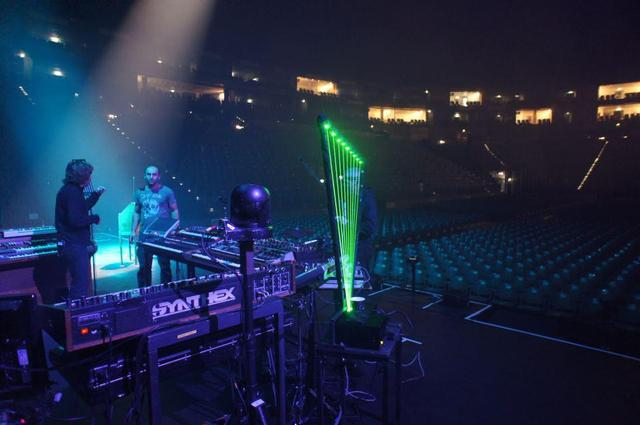
\includegraphics[width=\textwidth]{images/mini_harp.jpg} 
%\end{center}
%\begin{fr}
%\caption{La mini harp de Jean-Michel Jarre}
%\end{fr}
%\begin{en}
%\caption{Jean-Michel Jarre's Miniharp}
%\end{en}
%\label{jarre}
%\end{figure}

\subsubsection{Alvaro Cassinelli -- \textit{Score Light} -- 2008}

\begin{fr}
\textit{Score Light} est un projet d'Alvaro Cassinelli dans lequel un petit faisceau laser suit les contours de formes posées sur une table (cf. \ref{fig:cassinelli}). 
Il est possible de bouger les formes et d'en ajouter pour modifier la trajectoire du faisceau laser. 
Ce dispositif s'appuie sur le développement d'un module laser de faible puissance associé à une caméra, dispositif similaire à ce que l'on peut trouver dans les douchettes lasers pour scanner les codes barres.
Ce projet préfigure le projet \textit{Laser Game} en cours de développement et où le laser est projeté sur le t-shirt du joueur et rebondit sur les motifs à la manière d'une bille de flipper.
\end{fr}

\begin{en}
\textit{Score Light} is an Alvaro Cassinelli's project where a small laser beam follows shapes drawn in real time or moved on a desk (cf. \ref{fig:cassinelli}).
This installation uses a small laser associated with a video camera to detect contours.
Alvara Cassinelli is currently working on \textit{Laser Game} project : the laser beam is projected on a T-shirt and bounce on small printed dots like a flipper ball.
The gamer should move himself to save the ball from falling down.
\end{en}

\begin{figure}[ht]
\begin{center}
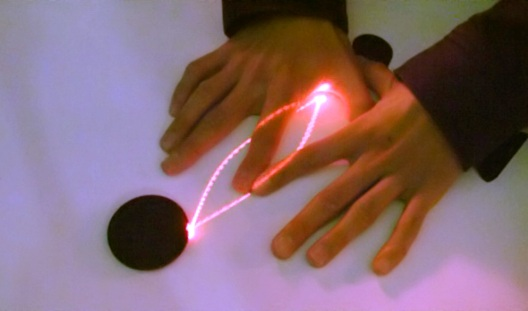
\includegraphics[width=\textwidth]{images/cassinellinews2.jpg} 
\end{center}
\caption{Alvaro Cassinelli -- \textit{Score Light}}
\label{fig:cassinelli}
\end{figure}

\subsubsection{Robin Fox -- \textit{Laser Show}}
\begin{fr}
Robin Fox utilise dans ses shows le laser comme un oscilloscope pour visualiser le signal audio qu'il génère en temps réel avec le logiciel Max/MSP. 
Il utilise la fumée pour matérialiser le faisceau et faire apparaître des volumes coniques dans l'espace (cf. \ref{fig:fox}).
Le show est impressionnant mais la corrélation systématique du son avec la visualisation le rend vite ennuyeux. 
Robin Fox utilise une carte son MOTU Traveller et un boîtier d'adaptation pour piloter son laser vert de 350\unit{mW} qu'il n'hésite pas envoyer dans les yeux du public.
\end{fr}

\begin{en}
Robin Fox uses laser like an oscilloscope.
He feeds the laser with the same signal he sends to loudspeakers.
This is generated by a Max/MSP patch in real-time.
Thanks to the smoke, the beam is visible in the space and volumes appears (cf. \ref{fig:fox}).
The beam scans the audience, this is dangerous even if the smoke attenuates the beam.
The show is impressive but the systematic correlation between sound and visual makes it boring quickly.
Robin Fox uses a MOTU Traveller sound card and a his own electronics to drive his 350\unit{mW} laser.
\end{en}

\begin{figure}[ht]
\begin{center}
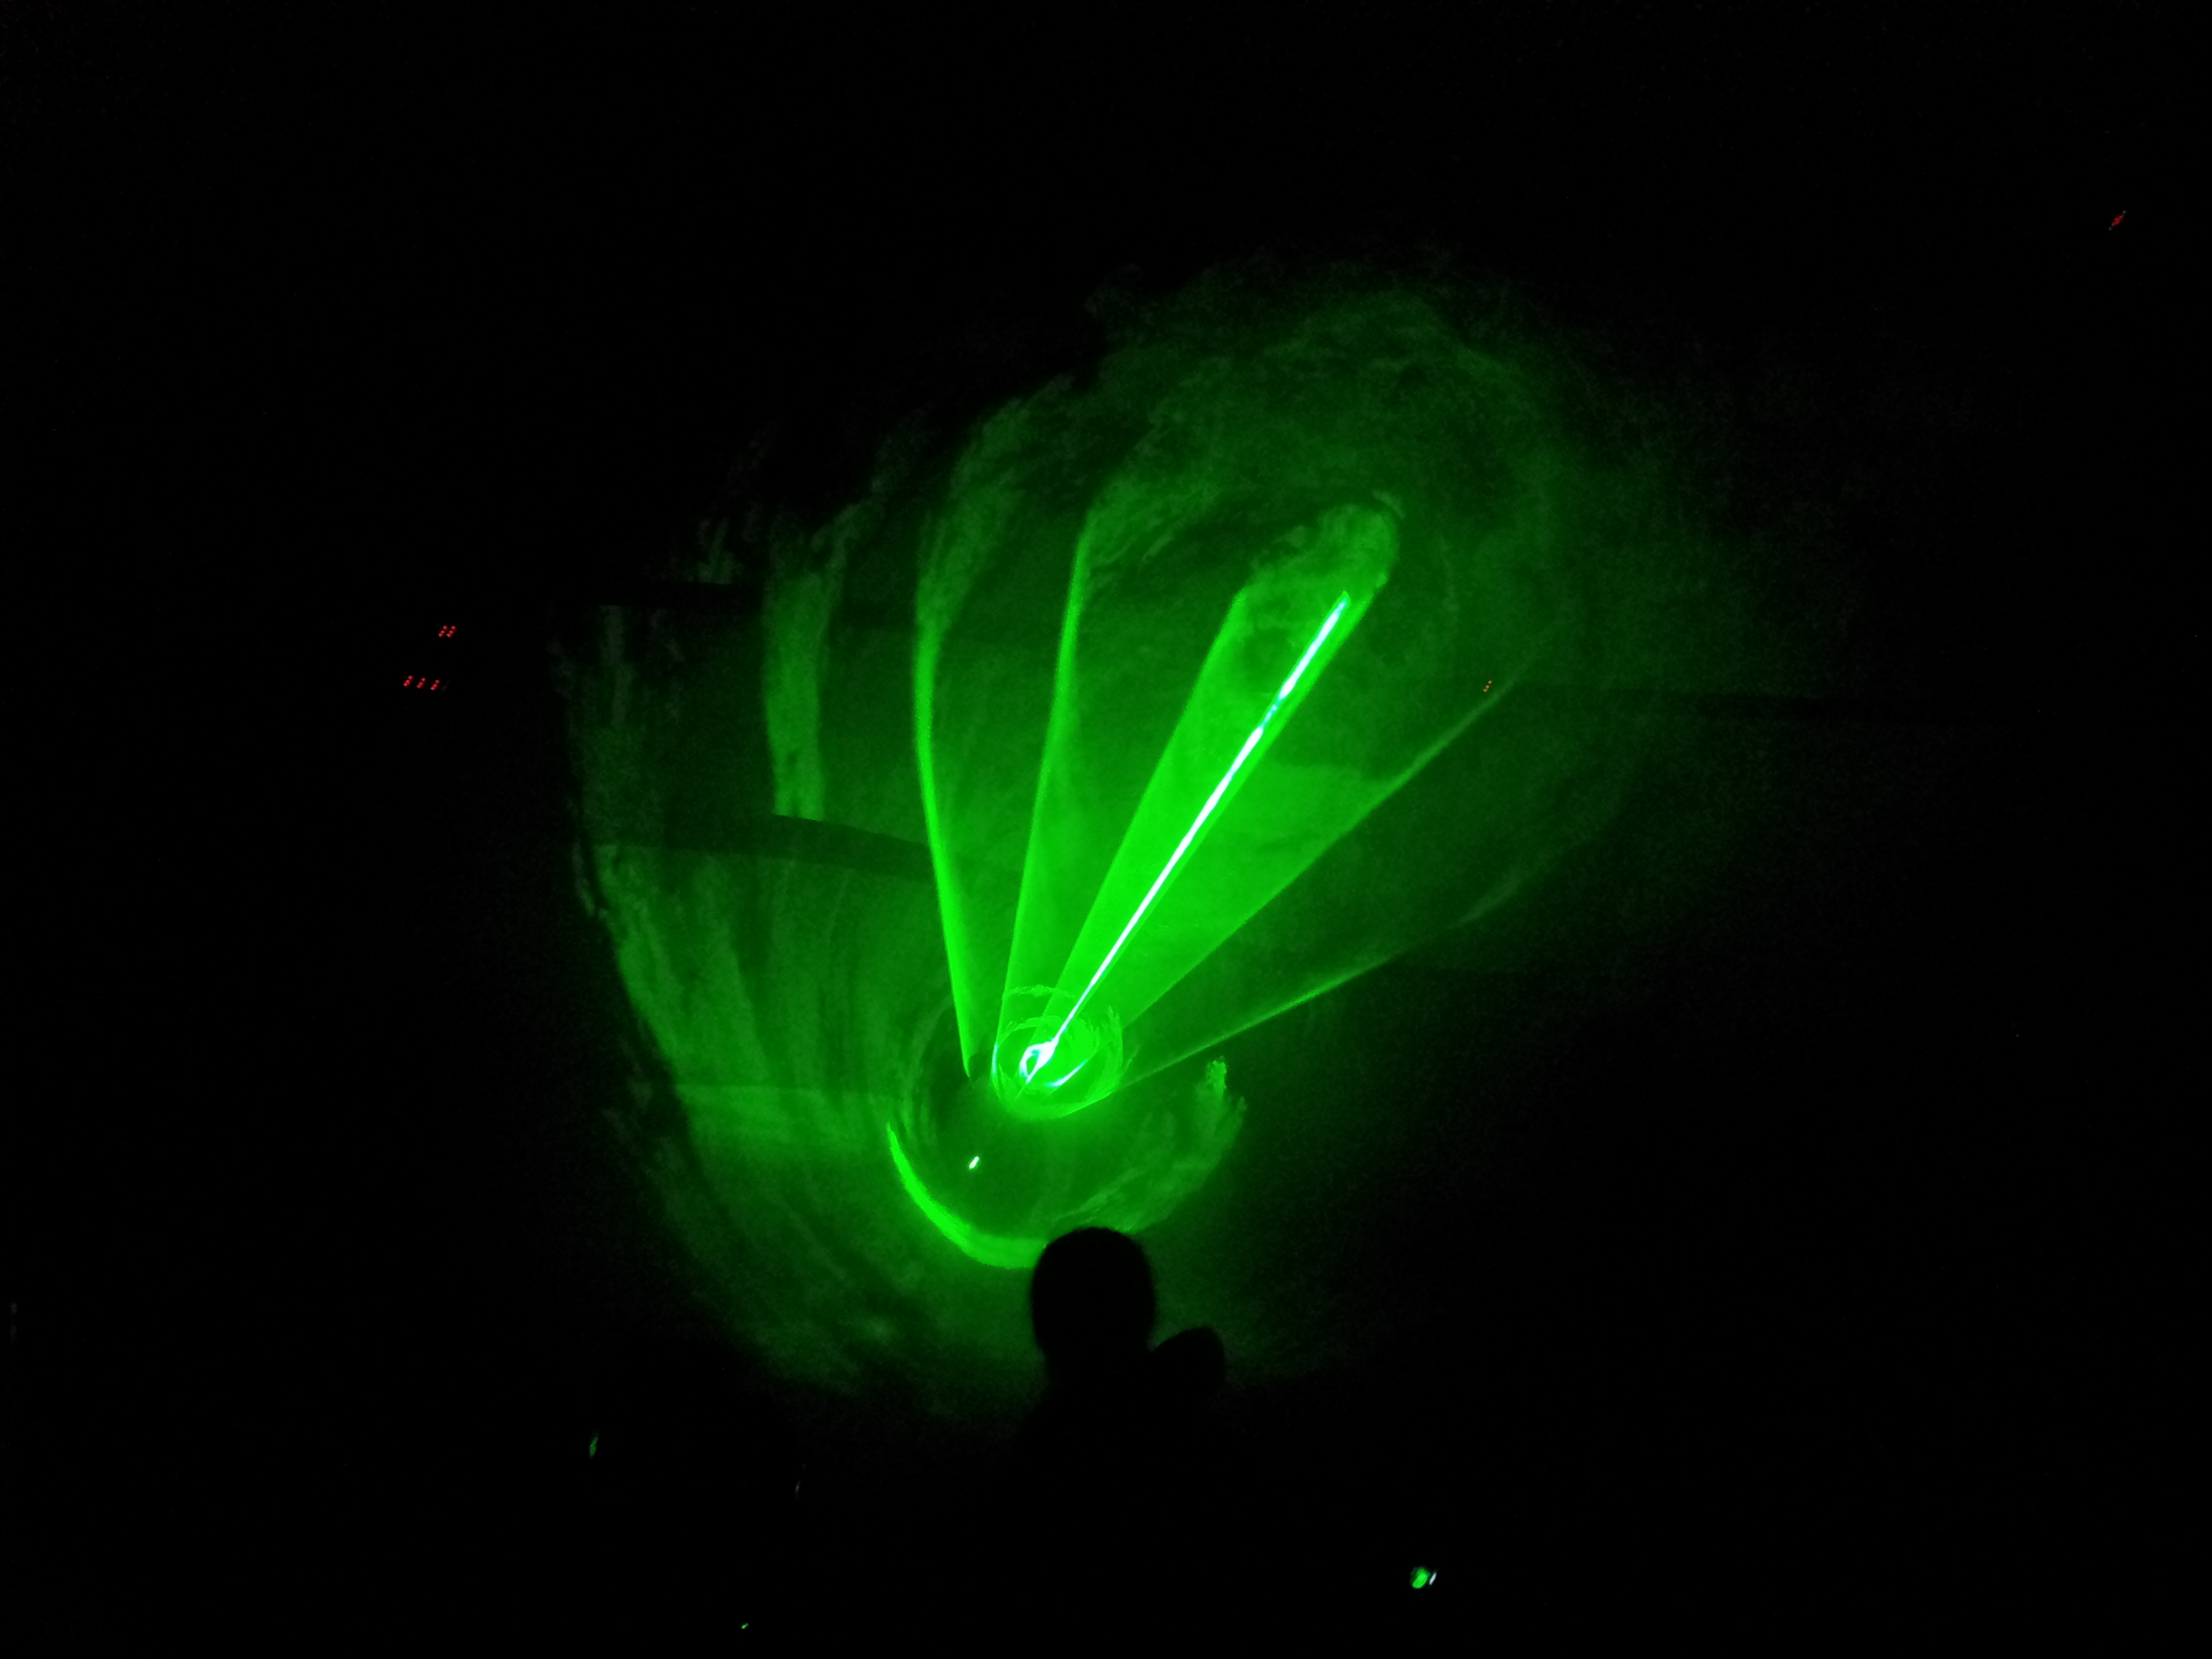
\includegraphics[width=\textwidth]{images/robin_fox.jpg} 
\end{center}
\caption{Robin Fox -- \textit{Laser Show}}
\label{fig:fox}
\end{figure}

\subsubsection{UVA -- \textit{Speed of light} -- 2010}
\begin{fr}
\textit{Speed of light} est un labyrinthe d'installations laser dans lequel les spectateurs sont invités à déambuler. 
Plusieurs installations présente des formes géométriques tissées à partir de quelques faisceaux lasers déviés par des miroirs fixes. 
Une autre affiche un texte de manière interactive.
Dans une interview on les voit travailler avec le logiciel Max/MSP, il est fort probable qu'ils l'aient utilisé pour piloter les lasers mais je n'ai pas pu le vérifier.
\end{fr}

\begin{en}
\textit{Speed of light} is a labyrinthic set of laser installations.
Several installations show volumic figures drawn with few lasers deflected thanks to fixed mirrors.
Another installation draws an interactive texte on a wall.
In a video, we show the team working with Max/MSP, they probably use this software to drive lasers, but I have no proof.
\end{en}

\begin{figure}[ht]
\begin{center}
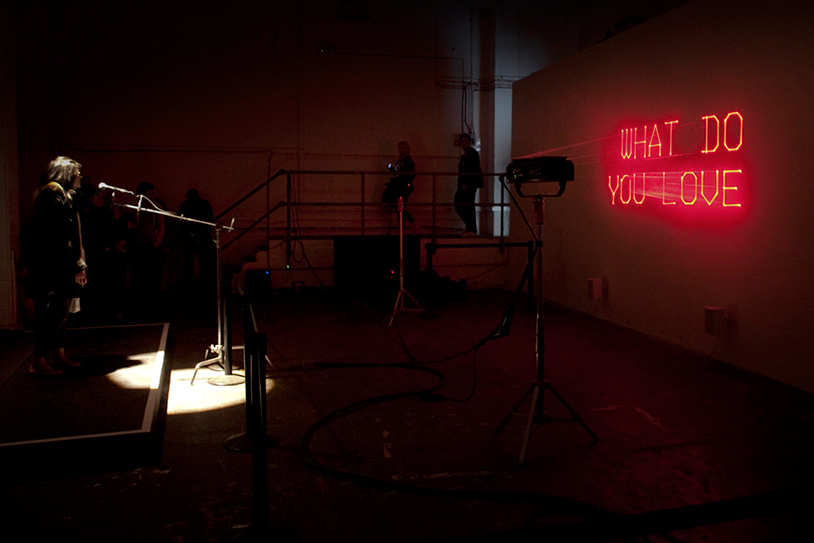
\includegraphics[width=\textwidth]{images/uva_sol_0121.jpg} 
\vskip 1em
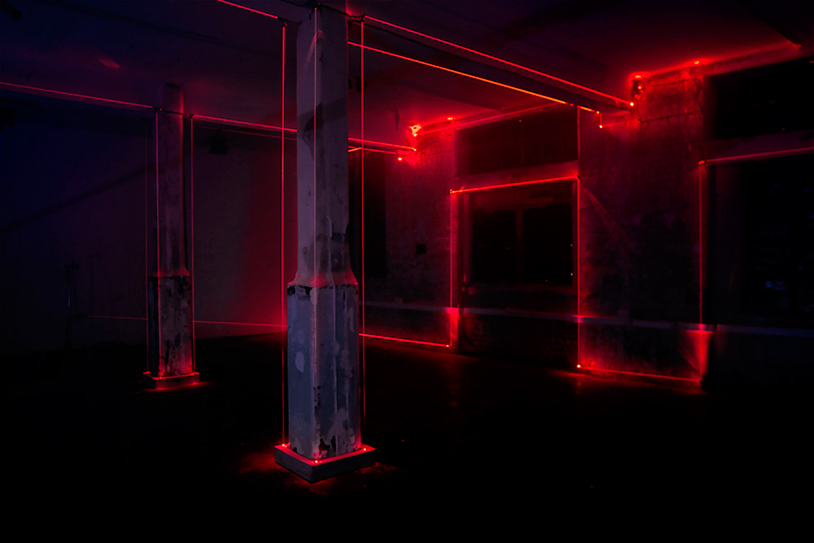
\includegraphics[width=\textwidth]{images/uva_sol_9181.jpg} 
\end{center}
\caption{UVA -- \textit{Speed of light}}
\label{fig:UVA}
\end{figure}

\subsubsection{Robert Henke -- \textit{Fragiles Territoires} -- 2012}
\begin{fr}
\textit{Fragiles territoires} est une installation interactive et générative de Robert Henke qui représente un réseau animé. Le public influe sur les algorithmes générant les formes géométriques et le son.
Cette installation a été présentée à l'espace LU de Nantes. 
Robert Henke utilise une carte son MOTU Traveller et quatre lasers bleu-jaunes de 5\unit{W}.
Face à la dangerosité de ces lasers et au fait de leur utilisation en intérieur, des mesures spéciales de sécurité ont été prises (cf. \ref{sec:legislation}).
\end{fr}

\begin{en}
\textit{Fragiles Territoires} is an interactive and generative installation by Robert Henke.
It shows an animated network.
The audience influences the audio and visual pattern generation.
This installation have been shown in \textit{Espace LU} in Nantes (FR).
Robert Henke uses a MOTU Traveller sound card to drive four yellow-blue 5\unit{W} lasers.
Due to the hazard of those powerful lasers and the indoor use, he deploys some special security measures (please refer to Appendix \ref{sec:legislation} to learn more).
\end{en}

\begin{figure}[ht]
\begin{center}
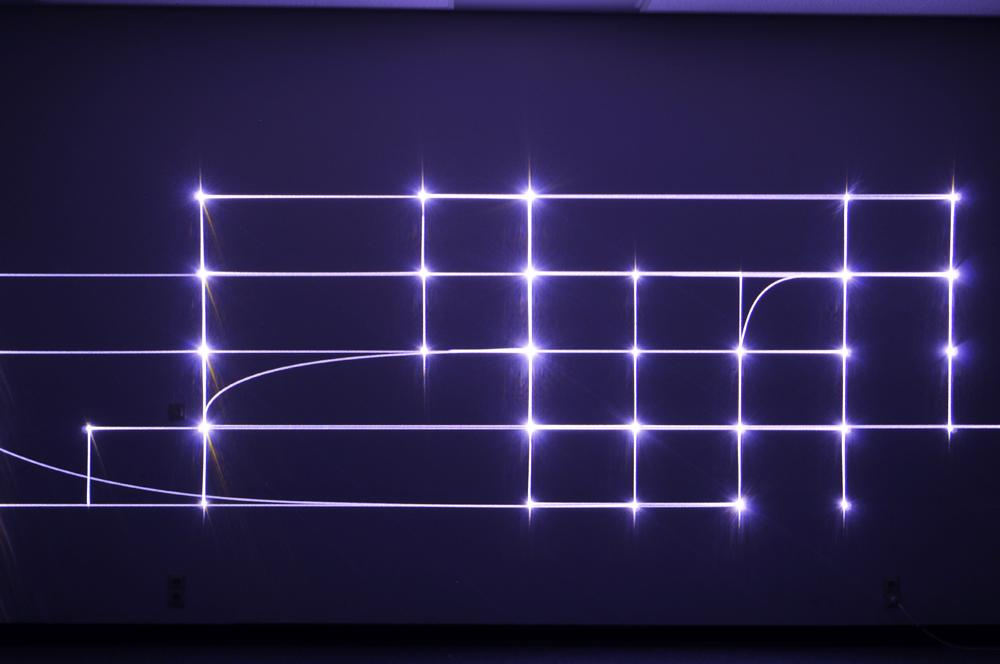
\includegraphics[width=\textwidth]{images/FragileTerritories.jpg} 
\end{center}
\caption{Robert Henke -- \textit{Fragiles Territoires}}
\label{fig:henke}
\end{figure}

\begin{fr}
\subsubsection{Samuel Bianchini -- \textit{Enseigne} -- 2012}
\textit{Enseingne} est une installation générative de Samuel Bianchini. Des mots issus du lexique scientifique et tirés des sites internet des lieux d'enseignement supérieur sont projetés à l'aide d'un laser sur la façade d'un bâtiment.
Les mots sont écrits dynamiquement avec une calligraphie manuscrite, des ratures, des hésitations, des barrés comme si quelqu'un était entrain d'écrire en temps réel.
Cette installation utilise un laser vert de 10\unit{W} piloté par une interface Galaxy Laser Show.
Un logiciel a spécialement été développé pour pouvoir piloter cette interface depuis Puredata (cf. \ref{sec:interfaces_ILDA} et figure \ref{fig:bianchini}).
\end{fr}

\begin{en}
\subsubsection{Samuel Bianchini -- \textit{Sign} -- 2012}
\textit{Sign} is a generative installation. Words taken from the scientific vocabulary and from the university website are written with a green laser on the front of a building.
The words are drawn with a handwritten calligraphy with hesitations and crossing out as if someone were currently writing on a pen tablet.
This installation uses a 10\unit{W} green laser driven by a Galaxy Show interface.
A software have been developed to use this interface with Puredata under Linux (cf. \ref{sec:interfaces_ILDA} and figure \ref{fig:bianchini}).
\end{en}
\begin{figure}[ht]
\begin{center}
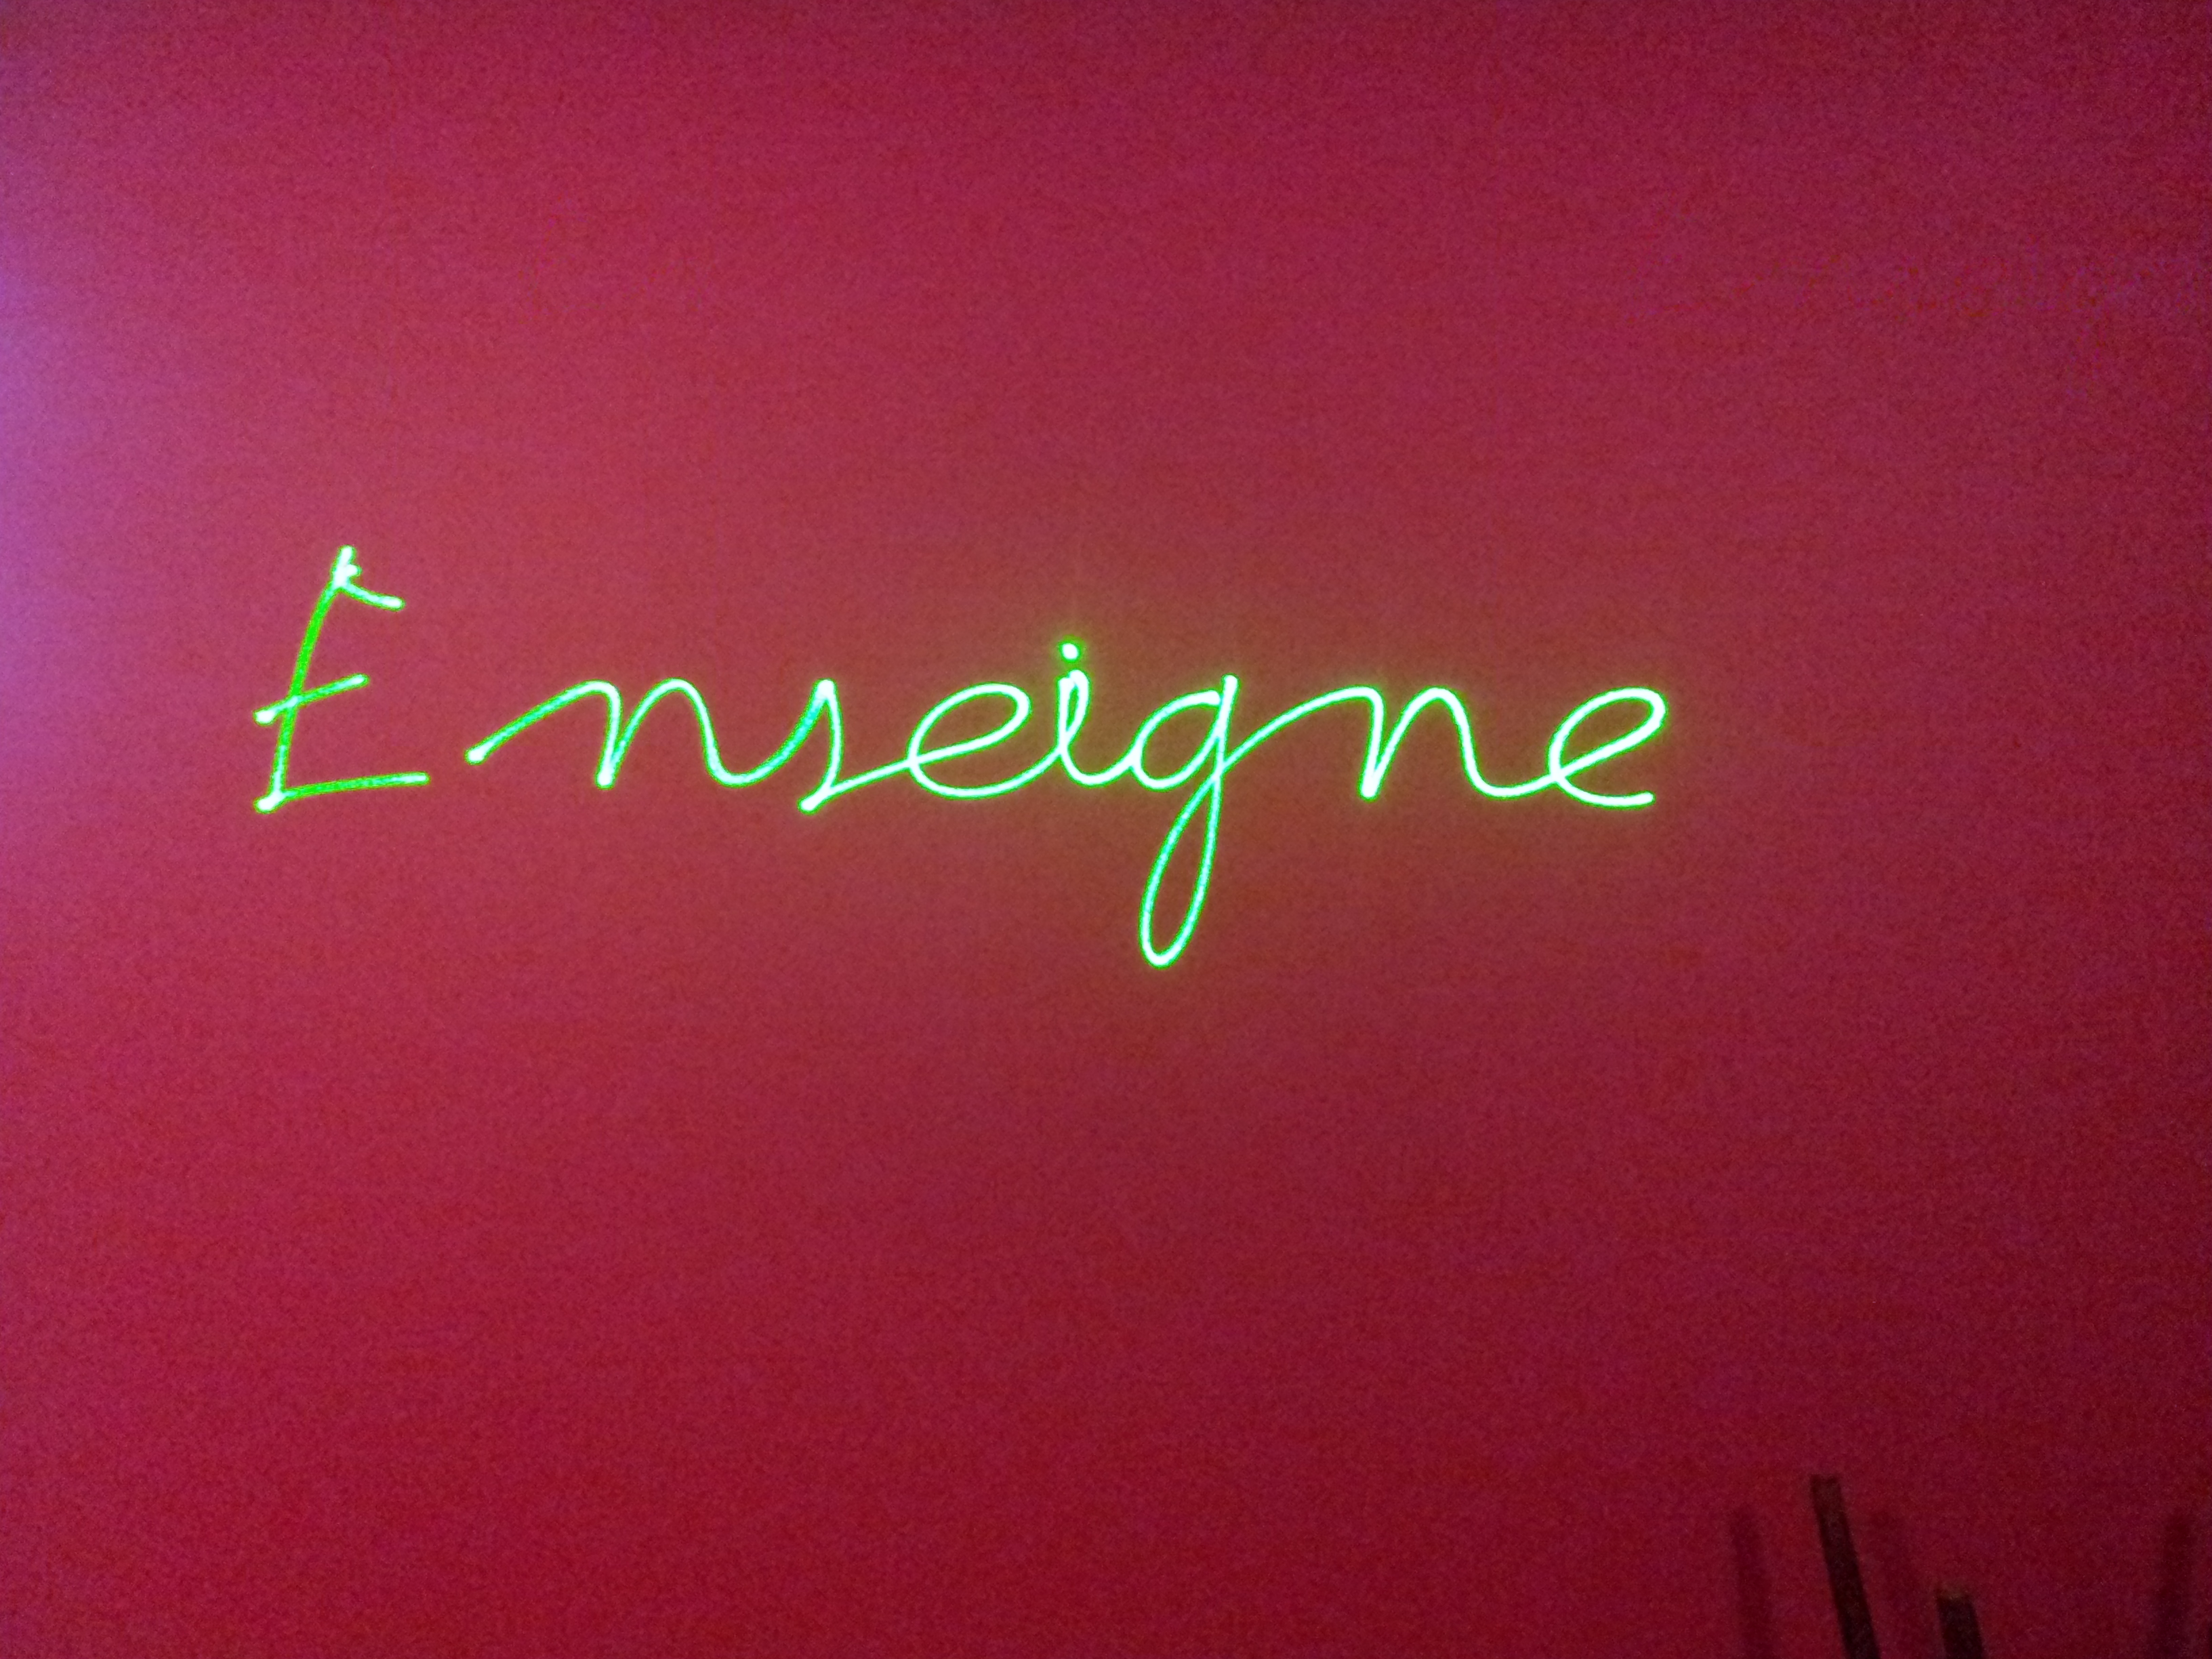
\includegraphics[width=\textwidth]{images/enseigne.jpg} 
\end{center}
\begin{fr}
\caption{Samuel Bianchini -- \textit{Enseigne}}
\end{fr}
\begin{en}
\caption{Samuel Bianchini -- \textit{Sign}}
\end{en}
\label{fig:bianchini}
\end{figure}

\subsubsection{Hyundai and WhiteVoid -- \textit{Fluidic - Sculpture in motion} -- 2013}
\begin{fr}
Pour la semaine du design de Milan, Hyundai a présenté au musée temporaire du nouveau design l'installation \textit{Fluidic - Sculpture in motion}.
Cette installation interactive utilise un système de captation tridimensionnel du mouvement pour que les spectateurs interagissent avec un nuage de millier de balles de ping-pong illuminé par de puissants laser bleus (cf. figure \ref{fig:fluidic}).
\end{fr}

\begin{en}
For the Milan's designer week 2013, Huyndai introduces \textit{Fuildic - Sculpture in motion}, an interactive installation made by Whitevoid team.
It uses a 3-dimensional motion capture disposal to track people gesture and to animate laser pattern projected on a cloud of thousand of ping-pong like balls (cf. figure \ref{fig:fluidic}).
\end{en}

\begin{figure}[ht]
\begin{center}
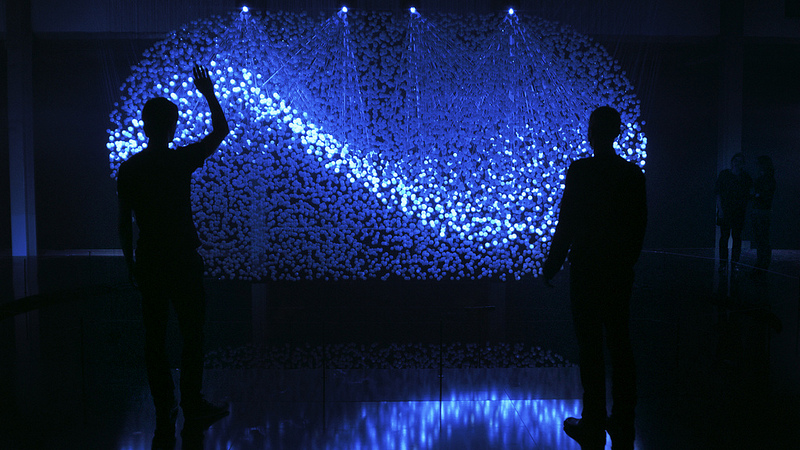
\includegraphics[width=\textwidth]{images/fluidic.jpg}
\end{center}
\caption{Hyundai and WhiteVoid -- \textit{Fluidic - Sculpture in motion}}
\label{fig:fluidic}
\end{figure}


\subsubsection{Daito Manabe -- \textit{UV laser fade out} -- 2010}
\begin{fr}
Daito Manabe utilise le laser dans plusieurs de ces projets.
\textit{UV laser fade out} utilise un laser ultra-violet pour dessiner sur un support phosphorescent. 
Le laser charge des petites surfaces successivement, la décharge progressive crée des niveaux de luminosité différents et fait apparaître une image (cf. figure \ref{fig:uv_laser_fadeout}).

Dans \textit{Pulse}, Daito Manabe utilise des lasers montés sur des bras robotisés et des miroirs placés dans tout l'espace pour dévier les trajectoires et créer un jeu de lumière.
\end{fr}

\begin{en}
Daito Manabe uses laser in several of his works.
\textit{UV laser fade out} involves a UV laser to draw on a phosphorescent board.
The laser charges successively small points, the discharge makes different luminosity levels and a picture appears (cf. figure \ref{fig:uv_laser_fadeout}).

With \textit{Pulse}, Daito Manabe uses laser mounted on robot and mirrors placed in a large space to deflect beams.
\end{en}

\begin{figure}[ht]
\begin{center}
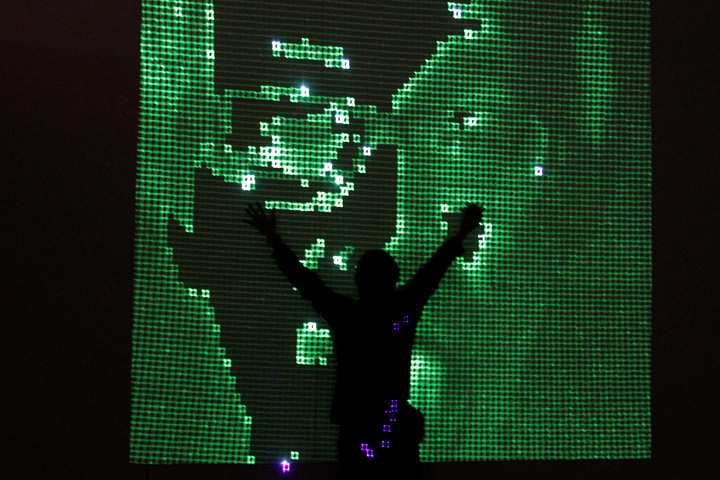
\includegraphics[width=\textwidth]{images/UV_laser_fadeout.jpg} 
\end{center}
\caption{Daito Manabe -- \textit{UV laser fade out}}
\label{fig:uv_laser_fadeout}
\end{figure}

\subsubsection{Antoine Villeret -- \textit{Silhouette} -- 2013}


\begin{fr}
\textit{Silhouette} est une installation interactive dans laquelle un projecteur laser dessine les silhouettes animées des spectateurs.
Lorsqu'un spectateur passe devant la caméra un trait vert apparaît au mur. S'il avance, le trait devient forme et le spectateur se reconnaît alors. 
Lorsqu'un spectateur passe devant la caméra un trait vert apparaît au mur. S'il avance, le trait devient forme et le spectateur se reconnaît alors. 
Le dispositif attire les visiteurs qui sont curieux des formes animées projetées au mur (cf. \ref{fig:silhouette}). 
Lorsque le public est trop nombreux, les silhouettes s'entremêlent et deviennent abstraites, à tel point que certains ne rendent pas compte que c'est eux qui sont représentés. 
Lorsqu'il y a moins de monde, les silhouettes deviennent plus nettes. Pour autant, le spectateur ne réalise pas forcément qu'il est représenté en temps réel. 
Souvent, lorsqu'il s'en rend compte, un jeu avec le dispositif débute. Les spectateurs dansent, sautent, font des grimaces pour tester le dispositif et chercher ses limites.
Cette installation utilise un capteur Kinect pour extraire les silhouettes ainsi que l'interface décrite dans la suite de ce document pour piloter le laser.
\end{fr}

\begin{en}
Silhouette is an interactive installation in which a laser projector draws animated silhouettes. 
It was first showed during the open days of the ENSAD in January 25th and 26th, 2013.

The visitors entered the building through a sinous and narrow corridor. 
At its end, they saw a green shape and realized by getting closer that it was their contour projected on a paper screen by a laser (cf. \ref{fig:silhouette}).

This disposal uses a depth sensor (Kinect) that easily extracts the visitor’s silhouettes. 
Those silhouettes are then vectorised and sent to the laser thanks to the custom interface decribed in the report. 
The whole video processing is achieved with puredata thanks to custom externals.
\end{en}

\begin{figure}[ht]
\begin{center}
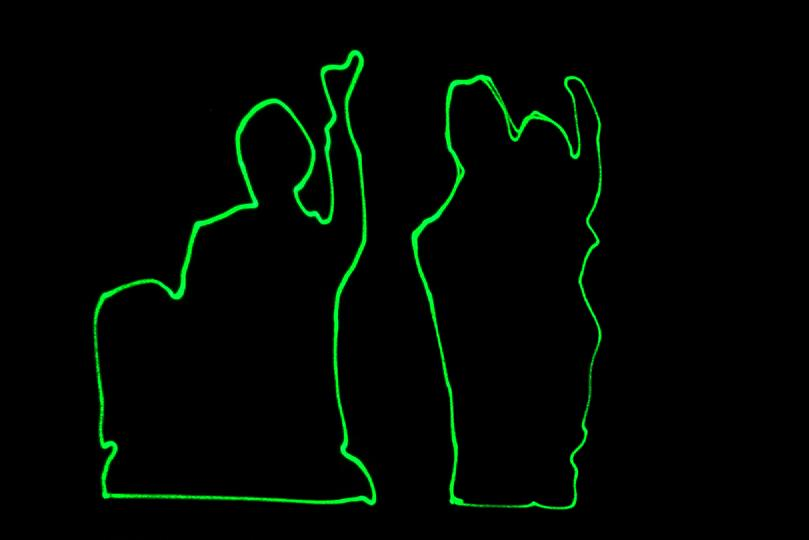
\includegraphics[width=\textwidth]{images/silhouette.jpg} 
\end{center}
\caption{Antoine Villeret -- \textit{Silhouette}}
\label{fig:silhouette}
\end{figure}

\subsubsection{Marshmallow Laser Feast -- \textit{Laser Forest} -- 2013}

\begin{fr} 
\textit{Laser Forest} utilise 150 lasers placés en haut de mâts d'environ 3\unit{m} constituant ainsi une « forêt ». 
La souplesse naturelle des mâts fait osciller les lasers dès lors qu'on les touche (cf. \ref{fig:laser_forest}). 
Ces lasers dessinent des formes mouvantes dans l'espace et à chaque « arbre » est associé un son.
\end{fr}

\begin{en}
\textit{Laser Forest} involves 150 lasers places on top of vertical 3\unit{m} tall metal tubes thus creating a "forest".
The natural springness of tube makes it oscillating when somebody touches it and then the laser draws figures on the ceiling (cf. \ref{fig:laser_forest}).
A tone is associated with each tree, visitors can play sound and light just by touching the tree.
\end{en}

\begin{figure}[ht]
\begin{center}
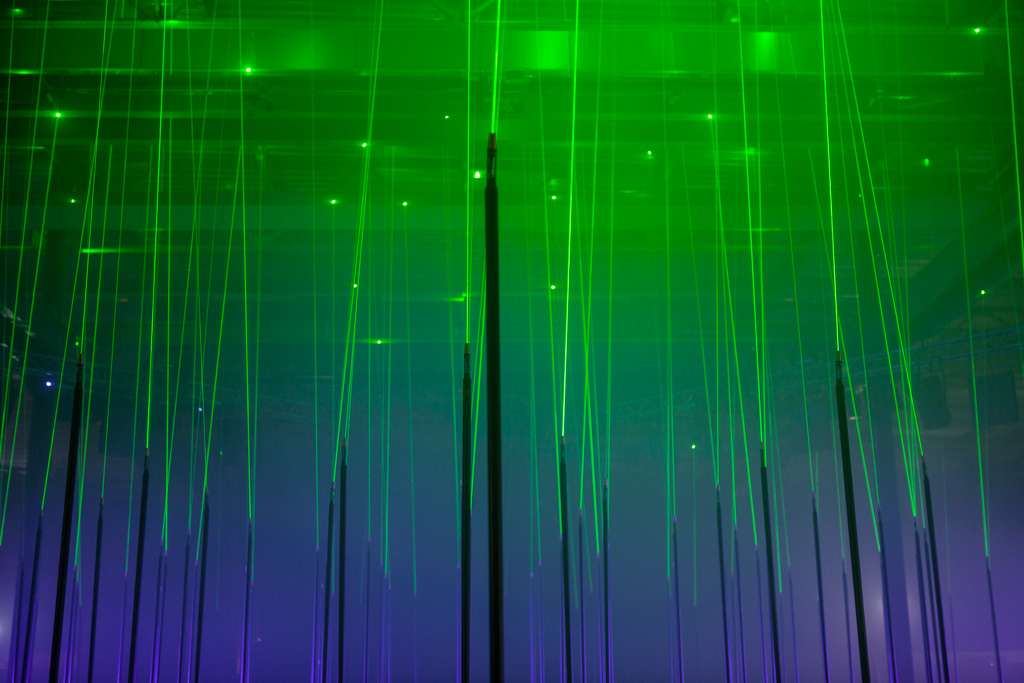
\includegraphics[width=\textwidth]{images/laser_forest-7.jpg}
\end{center}
\caption{Marshmallow Laser Feast -- \textit{Laser Forest}}
\label{fig:laser_forest}
\end{figure}

\clearpage

\begin{fr}
\subsection{État des techniques}
\end{fr}

\begin{fr}
\subsubsection{Un peu d'histoire}
Le laser a été conceptualisé par Albert Einstein vers 1917.
Le premier laser a été construit en 1958.
Son utilisation industrielle (découpe notamment) commence à la fin des années 70, depuis il est extrêmement utilisé : lecteur disque optique (CD, DVD...), lecteur de code barre, découpe de matériaux, arme de détection, capteur de distance\dots\ 
Jean-Michel Jarre fut, à ma connaissance, le premier à utiliser le laser dans un but artistique avec sa harpe laser.
\end{fr}

\begin{en}
\subsubsection{A bit of history}
The laser was conceptualized by Albert Einstein around 1917.
The first laser has been build around 1958.
Its industrial use starts in the late 70's, especially for cutting.
Since it is widely used in thousand of applications : optical drive, bar code reader, material cutting, weapon industry, distance sensor\dots
Jean-Michel Jarre was the first I know to use it in an artistic purpose with his laser harp.
\end{en}

\begin{fr}
\subsubsection{Les projecteurs d'animation}
Dans les projecteurs d'animation, le faisceau laser est dévié par des miroirs mobiles très rapides effectuant un balayage permanent.
La persistance rétinienne permet de voir la trace du laser.
Certains projecteurs sont dotés d'une entrée DMX qui permet de choisir le motif parmi une bibliothèque intégrée au projecteur et d'en modifier certains paramètres comme l'échelle ou la position. En revanche, le protocole DMX ne permet pas de dessiner des formes arbitraires. 
Pour cela, certains projecteurs sont équipés d'une entrée ILDA. 
Ce protocole analogique permet de contrôler directement les scanners et l'intensité des sources. On peut donc dessiner des formes arbitraires.
\end{fr}

\begin{en}
\subsubsection{Laser projectors}
Inside laser projectors, the beam is deflected by high speed moving mirrors.
The mirrors constantly scan the picture, thanks to the retinal persistence we saw a line and not a moving dot.
Some projectors have a DMX input but the DMX data could only choose pattern from a hard-coded library.
To draw arbitrary picture with a laser, we should drive the mirrors directly.
This is the aim of the ILDA protocol.
With this analog protocol, we can also control the intensity of the laser diode.
\end{en}

\begin{fr}
\subsubsection{Les interfaces ILDA}
\label{sec:interfaces_ILDA}
Bien que le protocole ILDA soit assez répandu sur les projecteurs d'animation à partir du milieu de gamme, il existe peu d'interfaces sur le marché permettant de les contrôler depuis un ordinateur.
\end{fr}

\begin{en}
\subsubsection{ILDA interfaces}
\label{sec:interfaces_ILDA}
Even if the ILDA protocol is widely used on laser projectors, there are only few solutions to drive them with a computer.
\end{en}

\begin{fr}
\paragraph*{Pangolin} Le leader du marché dans ce domaine est Pangolin qui propose une suite logicielle et matérielle complète pour contrôler les laser.
Au niveau logiciel, ils proposent des solutions pour réaliser de petits show laser (Quick Show) intégrant un séquenceur d'animation. 
Il propose également un SDK pour développer des applications spécifiques et des utilitaires de vectorisation pour convertir des images fixes.
Au niveau matériel, Pangolin a développé une chaîne technique très complète. On trouve des interfaces ILDA USB, réseau, OEM mais également des matrices permettant distribuer le signal à différents projecteurs et aussi des optiques spécifiques (pour projeter à 360\degres par exemple).

Malheureusement tout ceci est uniquement disponible pour Windows. 
Les solutions Pangolin sont assez onéreuses puisque l'interface avec le logiciel de base est commercialisée au prix de 650\,\euro\ et les versions professionnelles dépassent les 4\,000\,\euro .
\end{fr}

\begin{en}
\paragraph*{Pangolin} The world leader is Pangolin which has a complete technical chain from the software to the hardware.
On the software side, there are several solutions to make small shows or even huge ones.
There is also a SDK to develop custom software and some tools to vectorize bitmap images.

On the hardware side, there are ILDA interfaces with USB or Ethernet input and even an OEM solution to integrate the driver with another electronic device.
There are also devices to distribute ILDA signal between several projectors and a set of optical lenses to cover a 360° angle.

Unfortunately, those solutions are only available for Windows based computers and those are quite expensive.
The smallest device costs 650\euro\ and professional tools start around 4\,000\euro .
\end{en}

\paragraph*{Electro-concept}
\begin{fr}
Electro-concept\footnote{\url{http://www.boutique-electroconcept.com/boutique/}} a développé deux interfaces USB ILDA, Miniilda et Maxiilda commercialisées respectivement au prix de 219\,\euro\ et 349\,\euro .
Ces deux interfaces fonctionnent sous Windows uniquement.
J'ai pu testé l'interface Miniilda et j'ai développé un contrôleur avec Puredata. 
Mais l'interface manque de stabilité et Électro-concept est trop peu réactif à mes questions pour ce genre développement.
J'ai donc abandonné cette piste assez tôt.
\end{fr}

\begin{en}
Electro-concept\footnote{\url{http://www.boutique-electroconcept.com/boutique/}} developed two USB to ILDA interfaces, Miniilda and Maxiilda, respectively sold at \euro\,259 and \euro\,349.
Those two interfaces works under Windows with their own software.
I've tested the Miniilda which works under Linux thanks to a piece of software I've written.
Unfortunately it's not stable enough and Electro-concept doesn't appear to be interested in such a development.
So this way was early given up.
\end{en}

\paragraph*{Galaxy Laser Show}
\begin{fr}
Pour le projet \textit{Enseigne} de Samuel Bianchini (cf. \ref{fig:bianchini}), nous avons travaillé avec la société qui édite l'interface Galaxy Laser Show au dévelop\-pement d'un serveur cross-plateforme.
Ceci constituait une bonne initiative, même si le logiciel n'est pas open source, c'était la première interface qui fonctionne sous tous les systèmes d'exploitation que je connaisse.
L'interface est basé sur un serveur UDP programmé en C\# sur la plateforme .NET\footnote{.NET est une technologie de Microsoft qui est disponible sur Mac OS X et Linux à travers le framework open source Mono.} qui communique avec l'interface USB qui contient un FPGA.
Potentiellement, n'importe quel logiciel capable d'envoyer des données en UDP peut donc dessiner avec un laser et cette interface.

J'ai testé les versions 2 et 3 de l'interface Galaxy.
Avec la version 2, le serveur cesse de répondre lorsqu'on envoie des trames réseau trop petites ou lorsque la fréquence est trop élevée (au delà de 20\unit{kpps}).
Malgré ce problème, cette interface a été utilisée à plusieurs reprises pour la présentation d'\textit{Enseigne} et de la première version de mon installation \textit{Laser Drawer}.
Le modèle 3 que j'ai eu en test semble défectueux : l'interface n'est plus reconnue dès lors que quelque chose est reliée au connecteur SUB-D25.
\end{fr}

\begin{en}
For the \textit{Sign} project by Samuel Bianchini (cf. \ref{fig:bianchini}), we worked with Sonatronic, who produces the Galaxy Laser Show interface, to port it on Mac OS X and Linux.
This was a good initiative, even if the software source was not open, this is the first cross-platform interface I know.
It is based on a server written in C\# from the .NET framework\footnote{.NET is a Microsoft technology available on Mac OS X and Linux thanks to the open source Mono framework.}.
This server communicates with the interface which includes a FPGA.
Potentially any software capable of sending UDP packet can be used to draw with a laser projector.

I've tested the releases 2 and 3 of the interface.
With the revision 2, the software stops the communication with the hardware if network packets are too small or if scanners' frequency is above 20\unit{kpps}.
The version 3 I have to test was broken : as soon as something is plug in the Sub-D25 the interface is no more available to the software.
\end{en}

\begin{fr}
\paragraph*{Le projet bILDA \footnote{\url{}}}
bILDA est un projet d'interface laser open source constitué d'une interface électronique USB et d'un logiciel pour l'utiliser.
Ce projet est actuellement obsolète : le micro-contrôleur \texttt{AN2135SC} de Cypress Semiconductor, élément principal de la carte électronique, n'est plus fabriqué.
De plus, ses performances étaient assez modeste : les convertisseurs analogique-numérique \texttt{DAC0830} ont une quantification de 8\unit{bit} seulement.
\end{fr}

\begin{en}
\paragraph*{bILDA project}
bILDA is an open source USB to ILDA interface project.
It comes with an electronic board and a software.
This is unfortunately obsolete : the board is based on the chip \texttt{AN2135SC} from Cypress Semiconductor which is no more produced.
Moreover its performances were not very good : only 8\unit{bit} DAC.
\end{en}

\paragraph*{Etherdream\footnote{\url{http://ether-dream.com/}}}
\begin{fr}
        Etherdream est une interface ILDA Open Source extrêmement polyvalente.
        Elle possède une interface Ethernet permettant d'envoyer des trames ILDA jusqu'à 100\unit{kpps}.
        Son slot pour carte MicroSD permet de sauvegarder la configuration et de jouer des animations de manière autonome.
        Elle est entièrement configurable en OSC et intègre une correction de perspective.
        Je n'ai malheureusement découvert cette interface qu'après avoir conçu la mienne.
        Elles sont extrêmement similaires dans les foncitons disponibles.
        L'interface Etherdream est vendue 249\unit{\$}.
\end{fr}

\begin{en}
        Etherdream is an open source and versatile ILDA interface.
        It supports streaming playback over ethernet up to 100\unit{kpps}.
        All features can be controlled through OSC and it provides a perspective correction tool.
        It could run standalone thanks to its microSD card reader.
        Unfortunately I only discover this interface after designing my own one.
        The both provide similar functionnalities and are open source.
        Etherdream interface is available with case and power suppy for \$\,249.
\end{en}


\begin{fr}
\paragraph*{Les interfaces alternatives} Comme évoqué dans la partie \ref{sec:etat_de_l_art}, plusieurs artistes utilisent des cartes sons pour piloter les lasers. 
On retrouve à plusieurs reprise notamment la MOTU Traveller qui ne possède pas de filtres continus en sortie, ce qui permet d'envoyer un signal non symétrique par rapport à la masse et donc de décaler verticalement et horizontalement le dessin du laser par rapport au centre de la projection.
Ces artistes utilisent leur propre logiciel (souvent conçu à partir de Max/MSP) et leur propre interface d'adaptation du signal électrique.
\end{fr}

\begin{en}
\paragraph*{Alternative solutions} As is was seen in \ref{sec:etat_de_l_art}, several artists use sound card to drive laser and especially the MOTU Traveller.
This sound card has no DC filters on output so that we can produce an asymmetrical signal from the ground and thus translate the drawing horizontally or vertically from the projection center.
Those artists uses their own software (often made with Max/MSP) and their own electrical adaptation electronic.
\end{en}

\clearpage

\begin{fr}
\section{Le projet \textit{Laser Drawer}}
\subsection{Cahier des charges}
\paragraph*{Versatilité}
La première contrainte du dispositif est sa compatibilité avec les lasers d'animation du commerce. 
La norme ILDA défini un protocole analogique pour piloter ces lasers. 
Le dispositif doit donc être conforme à cette norme.
\end{fr}

\begin{en}
\section{The \textit{Laser Drawer} project}
\label{sec:laser_drawer_project}
\subsection{Specifications}
\paragraph{Versatility}
The most important thing is to be compatible with commercial laser projectors.
Those laser mostly use the ILDA protocol.
So that the interface should be ILDA compliant.
\end{en}

\begin{fr}
\paragraph*{Prix}
Les solutions (pack interface + logiciel) du commerce coûtent plusieurs centaines d'euros, \textit{Laser Drawer} est conçu à partir de matériel peu cher et d'un logiciel open source gratuit.
\end{fr}

\begin{en}
\paragraph*{Price}
Commercial solutions cost several hundred euros, \textit{Laser Drawer} should be cheap thanks to the use of widespread electronic devices and a free and open source software.
\end{en}

\begin{fr}
\paragraph*{Compatibilité}
\textit{Laser Drawer} est compatible avec la plupart des systèmes d'exploitation (Microsoft Windows, Apple Mac OS X, et les distributions Linux, notamment Debian et ses dérivés Ubuntu et Raspbian).
\end{fr}

\begin{en}
\textit{Laser Drawer} should work with most of operating system (Microsoft Windows, Apple Mac OS X, and Linux distros like Debian-based system (Ubuntu and Raspbian)).
\end{en}

\begin{fr}
\subsection{Conception}
Le dispositif \textit{Laser Drawer} se compose d'une partie matérielle et d'un logiciel pour la piloter.
\subsubsection{Matériel}
L'interface matériel de \textit{Laser Drawer} est basée sur une carte son et un étage d'adaptation à la norme ILDA.
\end{fr}

\begin{en}
\subsection{Software and hardware design}
\textit{Laser Drawer} has a hardware part and its associated software.
\subsubsection{Hardware}
The hardware part is based on a sound card and a electric adaptation board.
\end{en}


\begin{fr}
\paragraph*{Interface son}
La carte son ESI UDJ-6 a été choisie car elle est conforme à la norme USB Audio Class 1.0 et donc de fait compatible avec la plupart des systèmes (notamment Linux). 
Elle possède 6 sorties analogiques et aucune entrée, idéal pour piloter un laser tricolore. 
Elle fonctionne à une fréquence de 48\unit{kHz} en 24\unit{bit}, ce qui permet de piloter des scanners jusqu'à 48\unit{kpps} avec une grande précision.

Cette carte son possède des filtres de courant continu en sortie (DC filter) qu'il convient de supprimer pour pouvoir décaler le dessin par rapport à la position d'origine du laser. Pour ce faire, on court-circuite les condensateurs en soudant des fils comme indiqué en rouge sur la figure \ref{strap_DC}.
\end{fr}

\begin{en}
\paragraph*{Sound card}
I choose the ESI UDJ-6 sound card because it's USB Audio 1.0 compliant, thus it will run driver free on most current OS.
It has 6 analog outputs and no input, perfect to drive a RGB laser.
It runs at 48\unit{Hz} on 24\unit{bit} so it allows to drive laser up to 48\unit{kpps} with a very good precision.

This sound card has DC filter on output.
To remove them, it's just needed to short circuit some condensers by solder wire as shown in figure \ref{strap_DC}.
\end{en}

\begin{figure}[ht]
\begin{center}
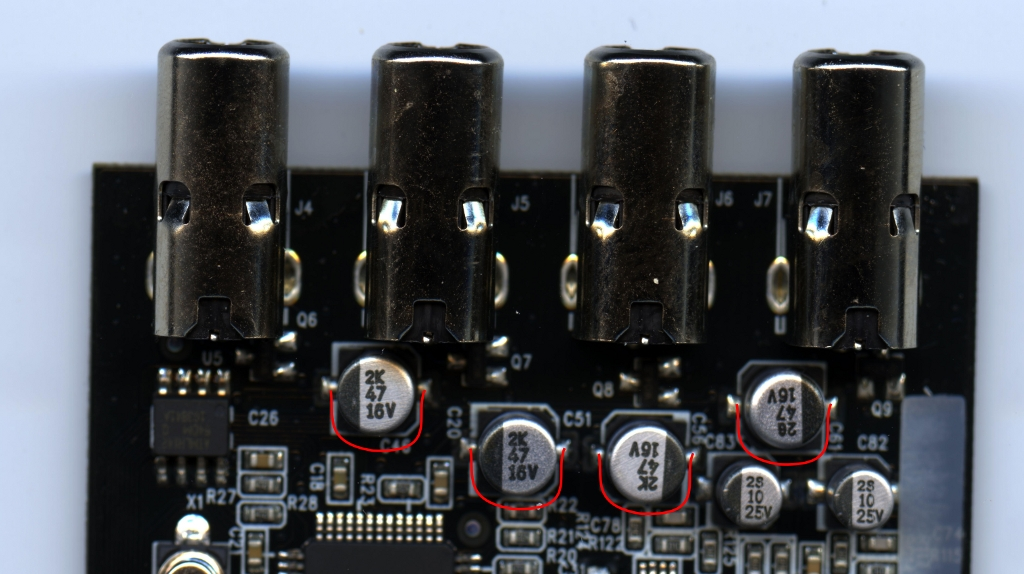
\includegraphics[width=0.75\textwidth]{images/strap_dc_removal.jpg} 
\end{center}
\begin{fr}
\caption{Filtre DC à court-circuiter}
\end{fr}
\begin{en}
\caption{DC filter bypassed}
\end{en}
\label{strap_DC}
\end{figure}

\begin{fr}
\paragraph*{Étage d'adaptation}
La carte son fournit un signal de 0,6\unit{V} crête à crête alors que la norme ILDA utilise des signaux de 10\unit{V} crête à crête.
Un étage d'adaptation est donc nécessaire pour amplifier le signal.
Pour des raisons pratiques, j'ai choisi d'alimenter cet étage d'adaptation directement depuis l'alimentation USB de la carte son (cela évite d'ajouter une alimentation externe). 
J'ai donc choisi un amplificateur opérationnel rail-to-rail permettant d'atteindre en sortie la valeur de la tension d'alimentation (ici 5 V). 
De plus le laser que j'avais à disposition pour réaliser ces développements n'est pas conforme à la norme ILDA, notamment l'entrée du signal ILDA n'est pas symétrisée. 
Pour que l'interface soit compatible avec ce laser, j'ai décidé de ne pas me conformer à la norme (pour la réalisation du prototype) et d'avoir des sorties asymétriques.

Ce choix a plusieurs conséquences. 
D'une part, le signal est plus sensible aux interférences, et donc il est nécessaire de réduire autant que possible les longueurs de câbles entre l'interface et le laser. 
D'autre part, seule la partie positive du signal a été gardée et donc au lieu d'avoir une tension crête-à-crête de 10\unit{V} comme préconisé par la norme, nous avons seulement 5\unit{V}. 
L'aire de balayage du laser est donc réduite de moitié.
A contrario, ce choix simplifie le montage électronique.
\end{fr}

\begin{en}
\paragraph*{Electrical adaptation stage}
The sound card deliver a 0.6\unit{V} peak-to-peak signal whereas the ILDA protocol requires 10\unit{V} peak-to-peak signals.
Then an electrical adaption stage is needed.
For practical reasons, I choose to power this stage directly from the USB power of the sound card.
I choose a rail-to-rail op-amp to reach the power supply value (5\unit{V}).
Moreover the laser projector I have is not really ILDA compliant (and yes, it's a pity) : the ILDA input is not balanced.
So I've decided to make the prototype not ILDA compliant but at least working with this projector.

This has several consequences.
First the signal is more sensitive to electro-magnetic perturbations, so the cable length should be as short as possible between the interface and the laser.
Then we keep only the positive part of the signal and instead of 10\unit{V} peak-to-peak we get only 5\unit{V}.
The scanning area is also divided by two but this simplifies the electronic.
\end{en}


\begin{fr}
\subsubsection{Logiciel}

Le logiciel qui pilote l'interface est un serveur OSC. 
Il reçoit les points sous forme de blobs\footnote{\texttt{blob} est un type de données OSC, un conteneur pour un bloc de données arbitraires} envoyés en un seul message.
Tous les blobs doivent avoir la même taille.
Les blobs correspondent respectivement aux canaux X, Y, rouge, vert et bleu.
Trois, quatre ou cinq blobs peuvent être envoyés simultanément, pour mettre à jour autant de tables.
Les paramètres de projection (échelle, taille, translation, vitesse...) sont quant à eux envoyés séparément avec un message OSC par paramètre. 
Le tableau \ref{tab:message_osc} donne les différents types de messages supportés par le serveur.
Les points sont stockés dans plusieurs tables qui sont ensuite lues, transformées selon les paramètres de la projection et envoyées à la carte son.
\end{fr}

\begin{en}
\subsubsection{Software}
The software is mainly an OSC server.
It receives points in several OSC blobs\footnote{\texttt{blob} is an OSC datatype with which we can transmit arbitrary data.} packed in one OSC message.
All blobs should have the same size.
They correspond respectively to channel X, Y, red, green and blue.
Three, four or five blobs should be send simultaneously to update as many tables.
The projections parameters are sent separately with one OSC message per parameter.
The table \ref{tab:message_osc} shows all supported messages.
Five tables keep the points in memory and then they are played and transformed according to projection parameters.
\end{en}


\begin{fr}
\begin{table}
\begin{bigcenter}
	\begin{tabular}{|l|p{2cm}|p{0.5\textwidth}|}
\hline 
\textbf{Message} & \textbf{Paramètre} \texttt{b : blob} \texttt{f : float} & \textbf{Effet} \\
\hline 
\texttt{/arrays} & \texttt{bbb\{b\}\{b\}} & Mise à jour des tables avec les données des blobs \\ 
\hline 
\texttt{/setting/offset} & \texttt{fff} & Décalage des canaux, respectivement X, Y et intensité \\ 
\hline 
\texttt{/setting/scale} & \texttt{fff} & Échelle respectivement en X, Y et intensité \\ 
\hline 
\texttt{/setting/invert} & \texttt{fff} & Inversion des canaux, respectivement X, Y et intensité \\ 
\hline 
\texttt{/setting/intensity} & \texttt{fff} & Intensité des canaux de couleur, respectivement R, G et B \\  
\hline
\texttt{/setting/blanking\_off} & \texttt{f} & Désactive le contrôle de l'intensité du laser \\
\hline
\texttt{/setting/angle\_correction} & \texttt{f} & Paramètre de correction d'angle (non implémentée pour le moment) \\
\hline
\texttt{/setting/end\_line\_correction} & \texttt{f} & Paramètre de correction de fin de ligne \\
\hline
\texttt{/setting/scan\_freq} & \texttt{f} & Fréquence en kHz des scanners \\
\hline
\texttt{/setting/perspective\_correction} & \texttt{f} & Active la correction de perspective \\
\hline
\texttt{/setting/dst\_point} & \texttt{ffffffff} & Points définissant l'espace de projection pour corriger la perspective \\
\hline
	\end{tabular}
	\end{bigcenter}
	\caption{\label{tab:message_osc} Messages OSC supportés par le serveur}
\end{table}
\end{fr}

\begin{en}
\begin{table}
\begin{bigcenter}
	\begin{tabular}{|l|p{2cm}|p{0.5\textwidth}|}
\hline 
\textbf{Message} & \textbf{Parameter} \texttt{b : blob} \texttt{f : float} & \textbf{Effect} \\
\hline 
\texttt{/arrays} & \texttt{bbb\{b\}\{b\}} & Update tables values \\ 
\hline 
\texttt{/setting/offset} & \texttt{fff} & Offset on each channel, resp. X, Y and intensity \\ 
\hline 
\texttt{/setting/scale} & \texttt{fff} & Scale on each cahnnel, resp. X, Y and intensity \\ 
\hline 
\texttt{/setting/invert} & \texttt{fff} & Invert each channel, resp. X, Y and intensity \\ 
\hline 
\texttt{/setting/intensity} & \texttt{fff} & Intensity on each color channel, resp. R, G and B \\  
\hline
\texttt{/setting/blanking\_off} & \texttt{f} & Turn off blanking \\
\hline
\texttt{/setting/angle\_correction} & \texttt{f} & Angle correction parameter (not implemented yet) \\
\hline
\texttt{/setting/end\_line\_correction} & \texttt{f} & End line correction \\
\hline
\texttt{/setting/scan\_freq} & \texttt{f} & Scanner frequency in \unit{kHz} \\
\hline
\texttt{/setting/perspective\_correction} & \texttt{f} & Turn perspective correction on and off \\
\hline
\texttt{/setting/dst\_point} & \texttt{ffffffff} & 4 corners coordinates to define projection area and to correct perspective \\
\hline
	\end{tabular}
	\end{bigcenter}
	\caption{\label{tab:message_osc} Handled OSC messages}
\end{table}
\end{en}

\begin{fr}
La correction de fin de ligne décale la lecture de la table d'intensité pour anticiper la latence d'allumage et d'extincition du laser.
Ceci considère toutefois que cette latence est constante, ce qui n'est pas vérifié.
\end{fr}

\begin{en}
The end line correction offsets the intensity table playhead by a small amount to compensate the diode switching latency.
This assumes the latency is constant but this was not verified.
\end{en}

\begin{fr}
Ce serveur, ainsi que le client associé, sont programmés en Puredata.
Tous deux dépendent de la bibliothèque \texttt{ILDA} de Puredata qui contient trois objets externes spécifiques à ce projet.
\texttt{ildasend} et \texttt{ildareceive} servent, respectivement, à envoyer et à recevoir les paquets OSC.
Ils dépendent de la bibliothèque \texttt{liblo}\footnote{\url{http://liblo.sourceforge.net/}}.
L'objet \texttt{ildafile}, basé sur \texttt{binfile} de Matin Peach, lit les fichiers d'animation \texttt{.ild} et charge leur contenu, trame par trame, dans une table que l'on peut ensuite envoyer au serveur.

L'architecture client/serveur OSC du logiciel permet de déporter le serveur sur une machine différente. 
Le serveur a été testé sur une Raspberry Pi. 
Malheureusement sur cette carte, le port ethernet est sur le même bus que les ports USB et lorsqu'on envoie des paquets trop grands, il y a des coupures dans la communication avec la carte son. 
Il en résulte des défauts visibles dans la trajectoire du laser.
Il est néanmoins pourtant peut être possible de faire fonctionner correctement cette interface modifiant les paramètres du driver (notamment en désactivant le mode turbo du contrôleur Ethernet) mais ces pistes n'ont pour l'instant pas été explorées.

Les sources du logiciel ainsi que les exemples sont disponibles sur mon github : \url{https://github.com/avilleret/laser_driver}.

\end{fr}

\begin{en}
The OSC server and its associated client are build in Puredata.
Both depend on the ILDA library for Puredata.
This library provides three externals and is part of the \textit{Laser Drawer} project.
The \texttt{ildasend} external formats and sends data over network whereas \texttt{ildareceive} receives and decodes them.
The \texttt{ildafile} external, based on \texttt{binfile} by Martin Peach, reads \texttt{.ild} files and load their content frame by frame into a table.

The server/client architecture allows to run each one on a separate computer.
I ran the server on Raspberry Pi but unfortunately I got crackles on sound and it results in artifacts in the drawing.
This is due to some issue on the internal firmware.
This could be fix by tuning some parameters like disabling the turbo mode of the Ethernet controller. 
But I didn't try it yet.

Software sources and examples are available on my github : \url{https://github.com/avilleret/laser_driver}.
\end{en}

\clearpage

\begin{fr}
\subsection{Comparaison avec l'interface Galaxy Laser Show}

Cette partie met en parallèle les performances de l'interface décrite ci-avant et de l'interface Galaxy Laser Show.
Pour cela, j'ai utilisé le motif de test et de réglage ILDA (cf. figure \ref{fig:ilda_pattern}) que j'ai observé à la fois à l'oscilloscope et projeté par le laser.
Ce pattern permet de régler les lasers en corrigeant la vitesse et l'amortissement des galvanomètres.
Sur la figure \ref{fig:ilda_pattern_proj} le cercle bleu apparaît projeté à l'intérieur du carré vert alors qu'il est situé à l'extérieur sur le dessin \ref{fig:ilda_pattern_vector}.
C'est ainsi qu'un laser bien réglé doit réagir d'après les recommandations de la norme ILDA.
\end{fr}

\begin{en}
\subsection{Laser Drawer vs. Galaxy Laser Show}

This section shows the performances of \textit{Laser Drawer} and \textit{Galaxy Laser Show} side by side.
I use the ILDA test pattern (cf. figure \ref{fig:ilda_pattern}) and observe it both with an oscilloscope and projected by the laser.
This pattern is used to tune projector by changing the high and low damping of galvanometers.
On the figure \ref{fig:ilda_pattern_proj} the blue circle appears inside the green square whereas on the vector image \ref{fig:ilda_pattern_vector} it appears outside.
This is how a well tuned laser should responds according to ILDA recommendation.
\end{en}

\begin{fr}
\begin{figure}[ht]
	\begin{bigcenter}
        \begin{subfigure}[b]{0.6\textwidth}
                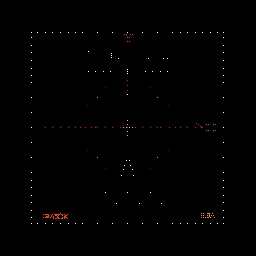
\includegraphics[width=\textwidth]{images/comp/ildatestpattern_256x256_point.jpg}
                \caption{Points}
                \label{fig:ilda_pattern_point}
        \end{subfigure}
        \begin{subfigure}[b]{0.6\textwidth}
                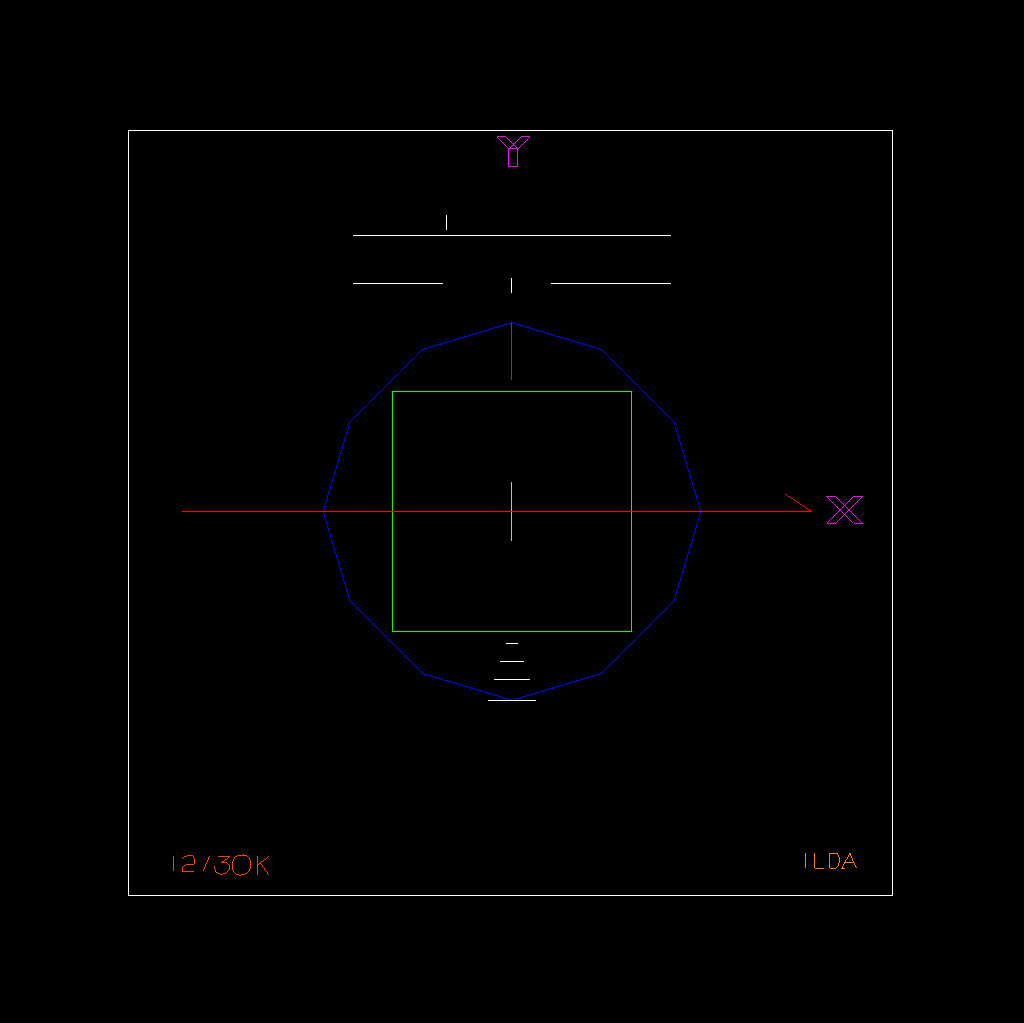
\includegraphics[width=\textwidth]{images/comp/ildatestpattern.jpg}
                \caption{Vecteurs}
                \label{fig:ilda_pattern_vector}
        \end{subfigure}
        
        \begin{subfigure}[b]{0.6\textwidth}
                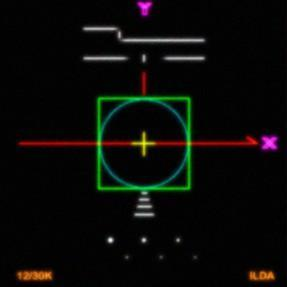
\includegraphics[width=\textwidth]{images/comp/mire_reference.jpg}
                \caption{Projeté avec un laser réglé}
                \label{fig:ilda_pattern_proj}
        \end{subfigure}     
	\end{bigcenter}
\caption{Points et vecteurs constituant le pattern de test ILDA}
\label{fig:ilda_pattern}
\end{figure}
\end{fr}

\begin{en}
\begin{figure}[ht]
	\begin{bigcenter}
        \begin{subfigure}[b]{0.6\textwidth}
                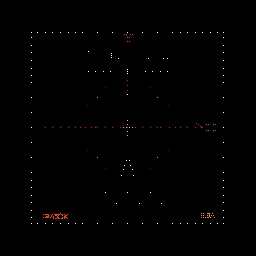
\includegraphics[width=\textwidth]{images/comp/ildatestpattern_256x256_point.jpg}
                \caption{Points}
                \label{fig:ilda_pattern_point}
        \end{subfigure}
        \begin{subfigure}[b]{0.6\textwidth}
                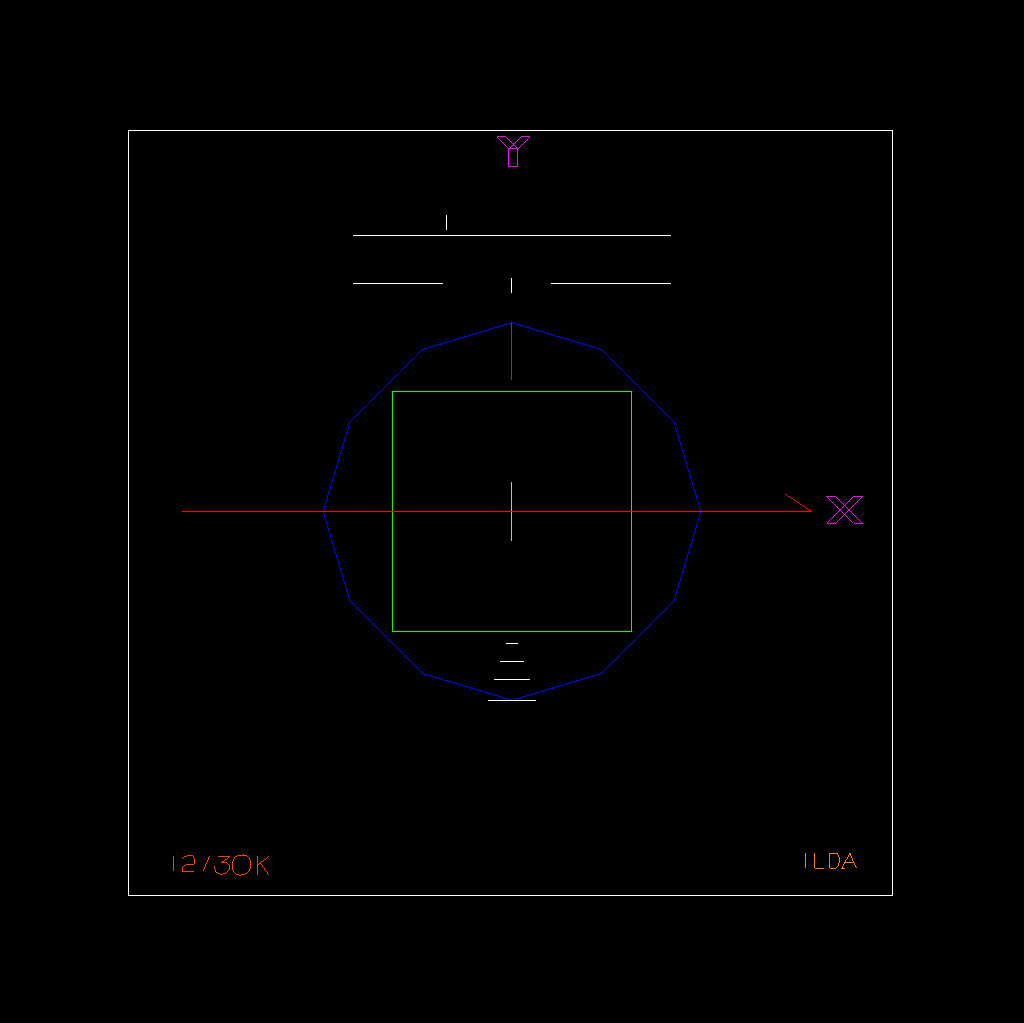
\includegraphics[width=\textwidth]{images/comp/ildatestpattern.jpg}
                \caption{Vectors}
                \label{fig:ilda_pattern_vector}
        \end{subfigure}
        
        \begin{subfigure}[b]{0.6\textwidth}
                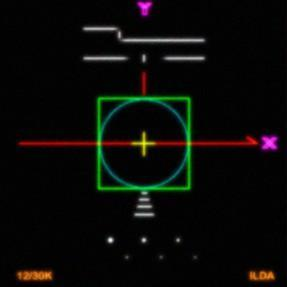
\includegraphics[width=\textwidth]{images/comp/mire_reference.jpg}
                \caption{Projected with a well tuned laser}
                \label{fig:ilda_pattern_proj}
        \end{subfigure}     
	\end{bigcenter}
\caption{ILDA pattern : points, vectors and reference projection}
\label{fig:ilda_pattern}
\end{figure}
\end{en}

\begin{en}
\end{en}


\begin{fr}
La première constatation est que l'interface Galaxy n'interpole pas de ma\-nière continue entre les points.
Sur la figure \ref{fig:ilda_pattern_point} on voit que le cercle bleu est constitué de douze points, sur la figure \ref{fig:galaxy_10k} il en possède trente alors que sur la figure \ref{fig:custom_10k} le cercle est continu.
Ceci est problématique pour deux raisons.
Tout d'abord on verra les points discrets au lieu d'un trait avec une diode extrêmement réactive. 
De plus, en rajoutant des points le tracé est faussé et le cercle apparaît en dehors du carré avec un laser bien réglé (cf. figure \ref{fig:proj_test_galaxy}).
\end{fr}

\begin{en}
The first observation is that Galaxy interface doesn't interpolate continuously between points.
We show only points, not lines.
On the figure \ref{fig:ilda_pattern_point}, the blue circle is made of 12 points whereas on the figure \ref{fig:galaxy_10k} there are 30 and on figure \ref{fig:custom_10k} the circle line is continuous.
This is an issue for two reasons.
First we will see points instead of lines with a low latency laser diode.
And then by adding points, the drawing is not right (according to ILDA recommendation), the circle appears outside of the square with a well tuned laser (cf. figure \ref{fig:proj_test_galaxy}).
\end{en}


\begin{figure}[ht]
	\begin{bigcenter}
        \begin{subfigure}[b]{0.5\textwidth}
                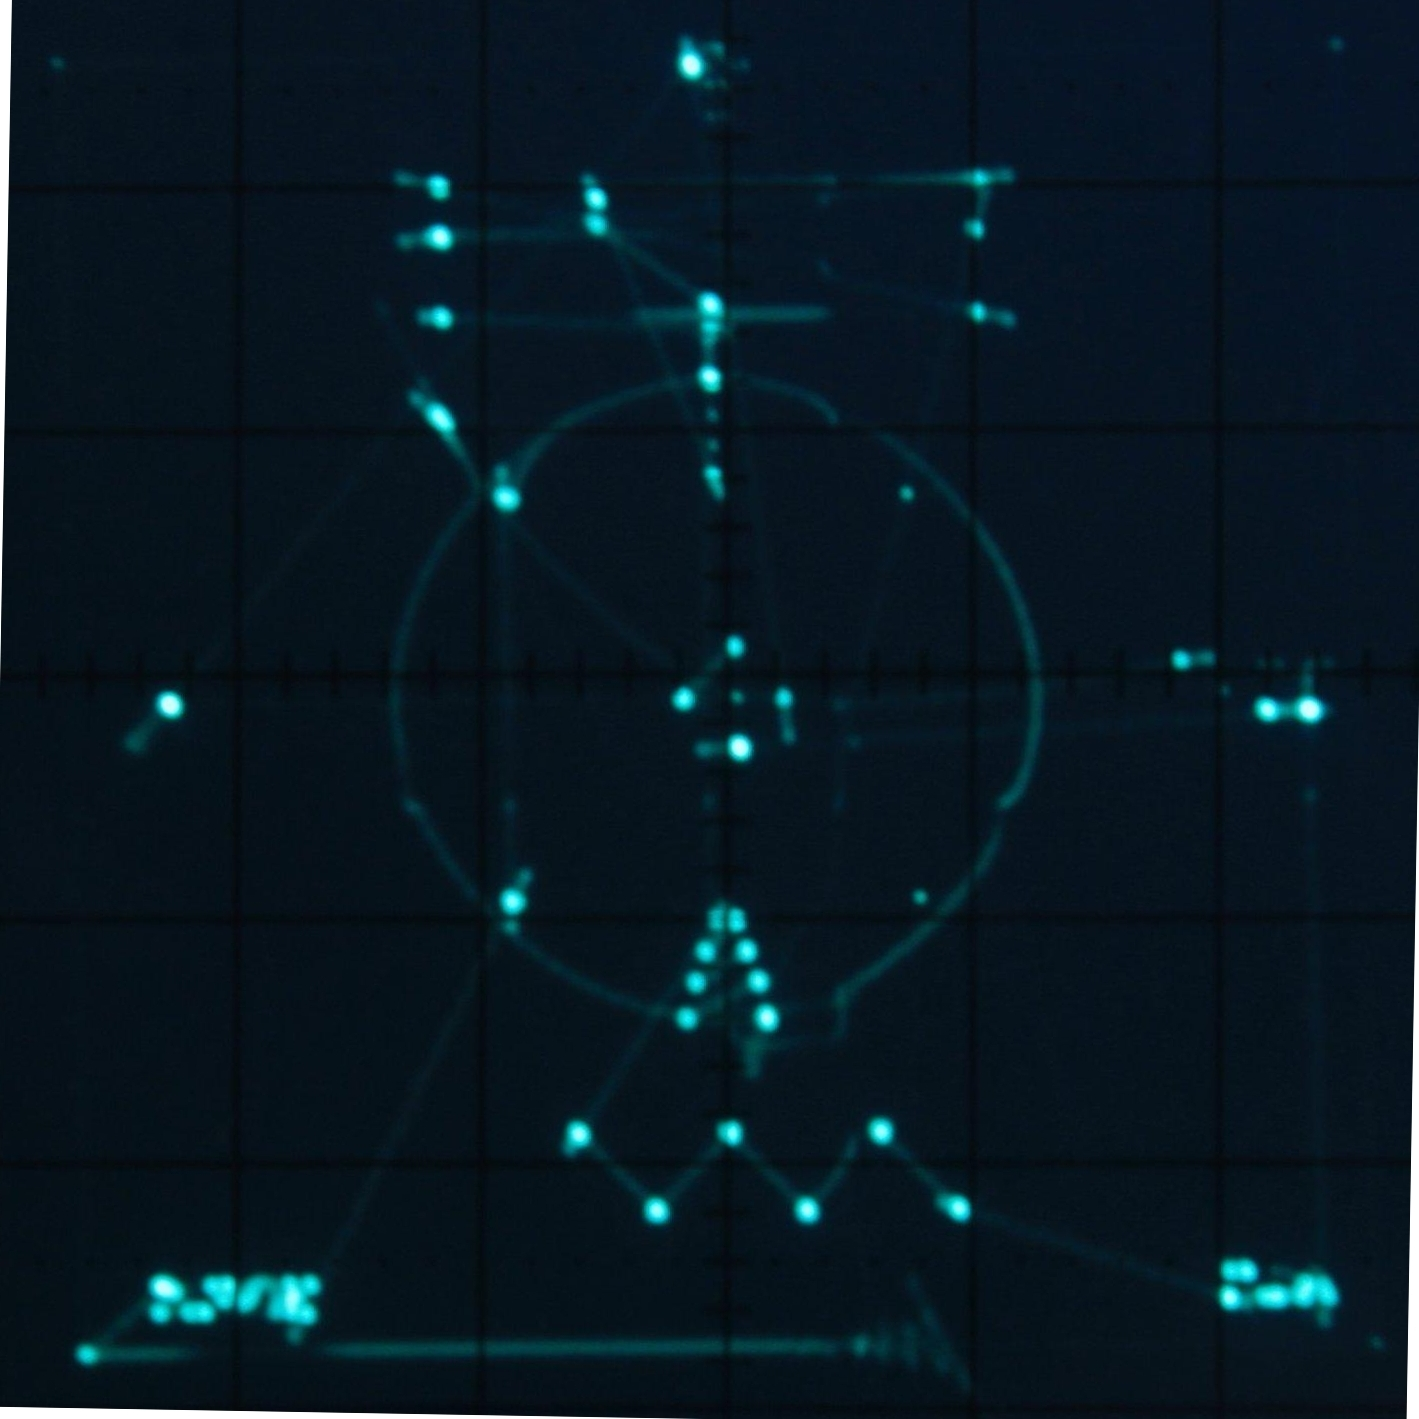
\includegraphics[width=\textwidth]{images/comp/custom_10k.jpg}
                \caption{Laser Drawer}
                \label{fig:custom_10k}
        \end{subfigure}
        \begin{subfigure}[b]{0.5\textwidth}
                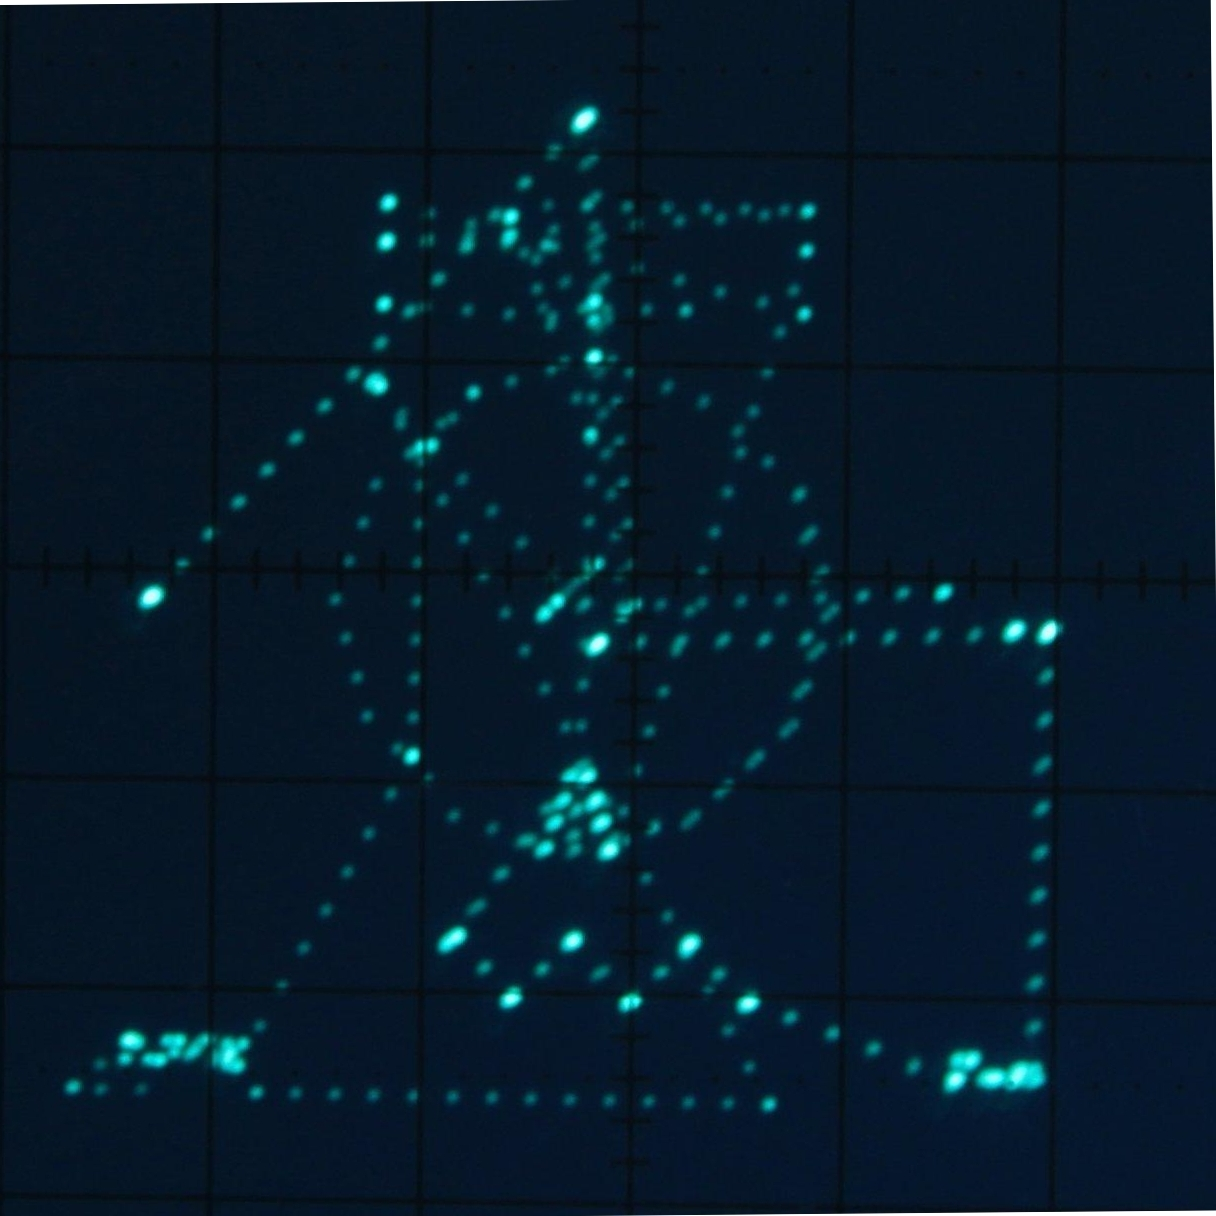
\includegraphics[width=\textwidth]{images/comp/galaxy_10k.jpg}
                \caption{Galaxy}
                \label{fig:galaxy_10k}
        \end{subfigure}       
	\end{bigcenter}
\begin{fr}
\caption{Observation à l'oscilloscope à 12\unit{kpps}}
\end{fr}
\begin{en}
\caption{On oscilloscope at 12\unit{kpps}}
\end{en}
\label{ildatestpattern_point}
\end{figure}

\begin{fr}
On constate sur la figure \ref{fig:test_osc_limit} que l'interface Galaxy est plus stable que la mienne. 
Néanmoins, il apparaît des points plus lumineux au fur à mesure que l'on augmente la vitesse.

Les défauts qui apparaissent sur le cercle de la figure \ref{fig:custom_48k} sont des non-linéarités des AOP dues à l'utilisation  de ceux-ci dans des conditions limites.
Lors des tests l'interface était alimentée depuis l'alimentation des scanners en +15\unit{V}/-15\unit{V}.
Les AOP \texttt{LM358} en place à ce moment là étaient donc utilisés dans des conditions limites car la tension d'alimentation mesurée de 31\unit{V} est proche de la limite théorique de 32\unit{V}.
L'utilisation d'autres AOP et d'une tension d'alimentation plus faible devrait règler ce problème.
\end{fr}

\begin{en}
The figure \ref{fig:test_osc_limit} shows \textit{Galaxy} is more stable than \textit{Laser Drawer's} when increasing scanners frequency.
But with \textit{Galaxy}, some point become lighter when increasing scanner frequency.

The small artifacts on the circle in figure  \ref{fig:custom_48k} are non-linearities of op-amp due to power supply reaching the op-amp's limits.
During the tests, the board was supplied by the laser's main 15\unit{V}/-15\unit{V}.
The \texttt{LM358} op-amp were about to fire.
The use of other op-amp and lowser power supply should fix this.
\end{en}



\begin{figure}[ht]
	\begin{bigcenter}
        \begin{subfigure}[b]{0.5\textwidth}
                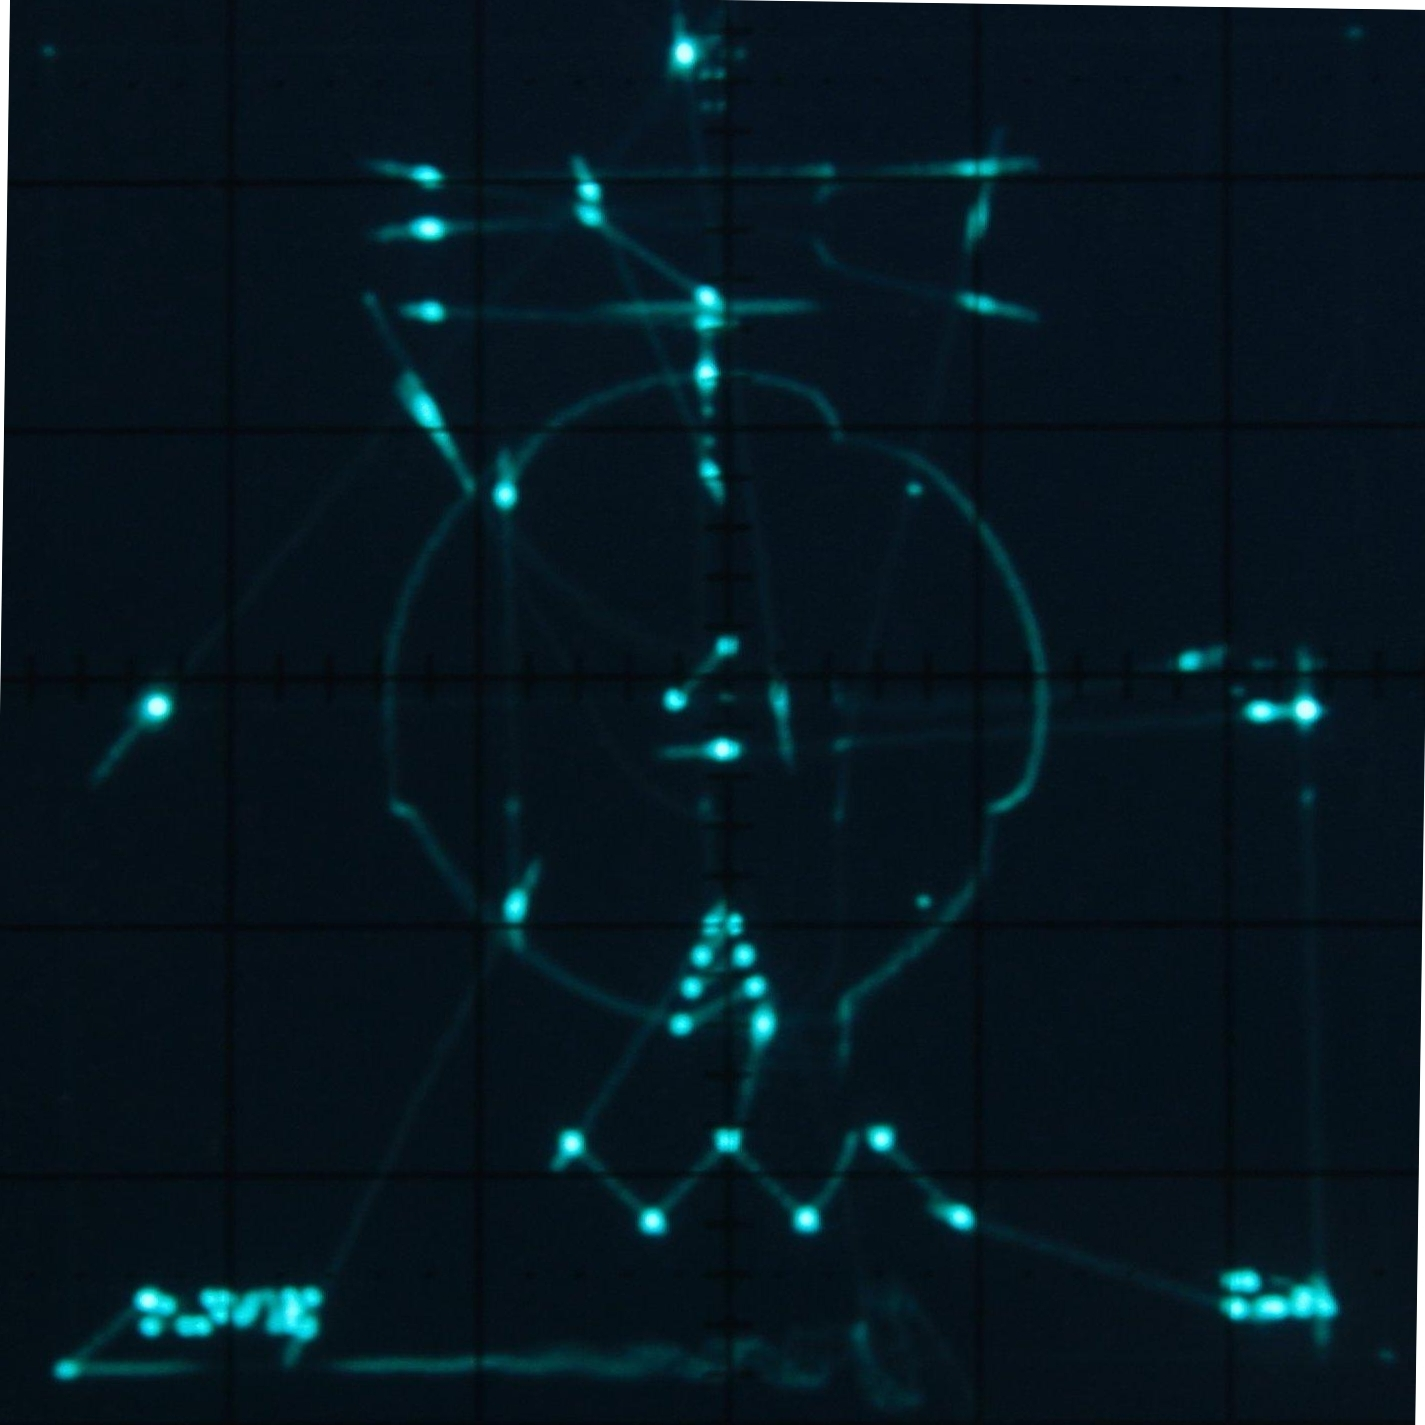
\includegraphics[width=\textwidth]{images/comp/custom_40k.jpg}
                \caption{Laser Drawer -- 48\unit{kpps}}
                \label{fig:custom_48k}
        \end{subfigure}
        \begin{subfigure}[b]{0.5\textwidth}
                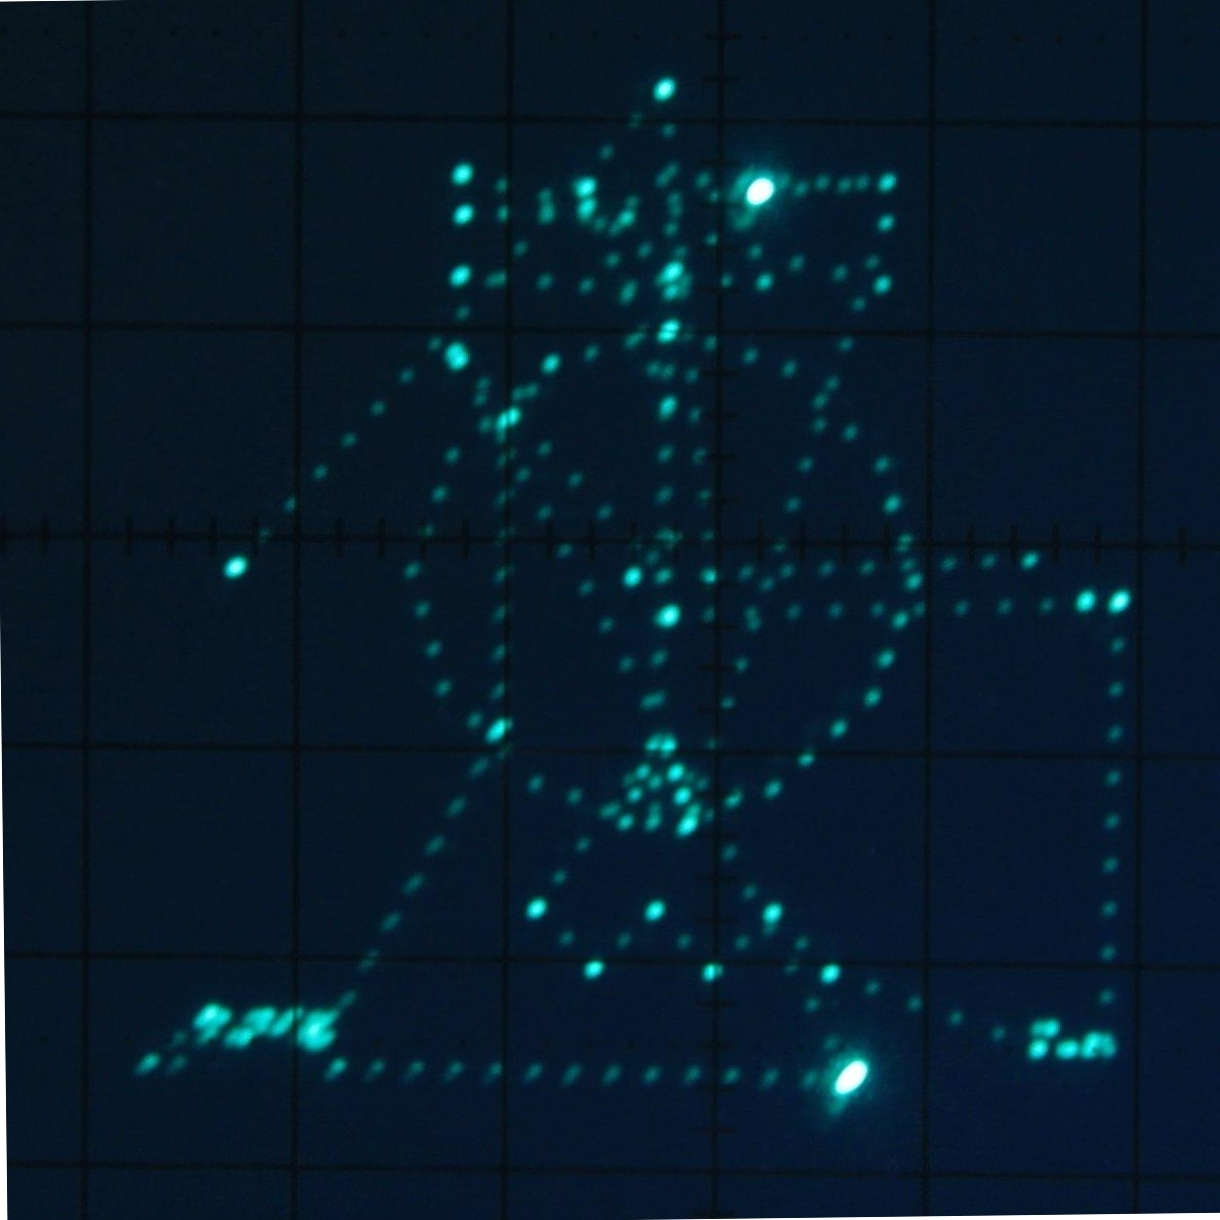
\includegraphics[width=\textwidth]{images/comp/galaxy_100k.jpg}
                \caption{Galaxy -- 100\unit{kkps}}
                \label{fig:galaxy_100k}
        \end{subfigure}       
	\end{bigcenter}
	\begin{fr}
	\caption{Observation à l'oscilloscope à la vitesse limite}
	\end{fr}
	\begin{en}
	\caption{Highest speed shown on oscilloscope}
	\end{en}
\label{fig:test_osc_limit}
\end{figure}



\begin{figure}[ht]
	\begin{bigcenter}
        \begin{subfigure}[b]{0.5\textwidth}
                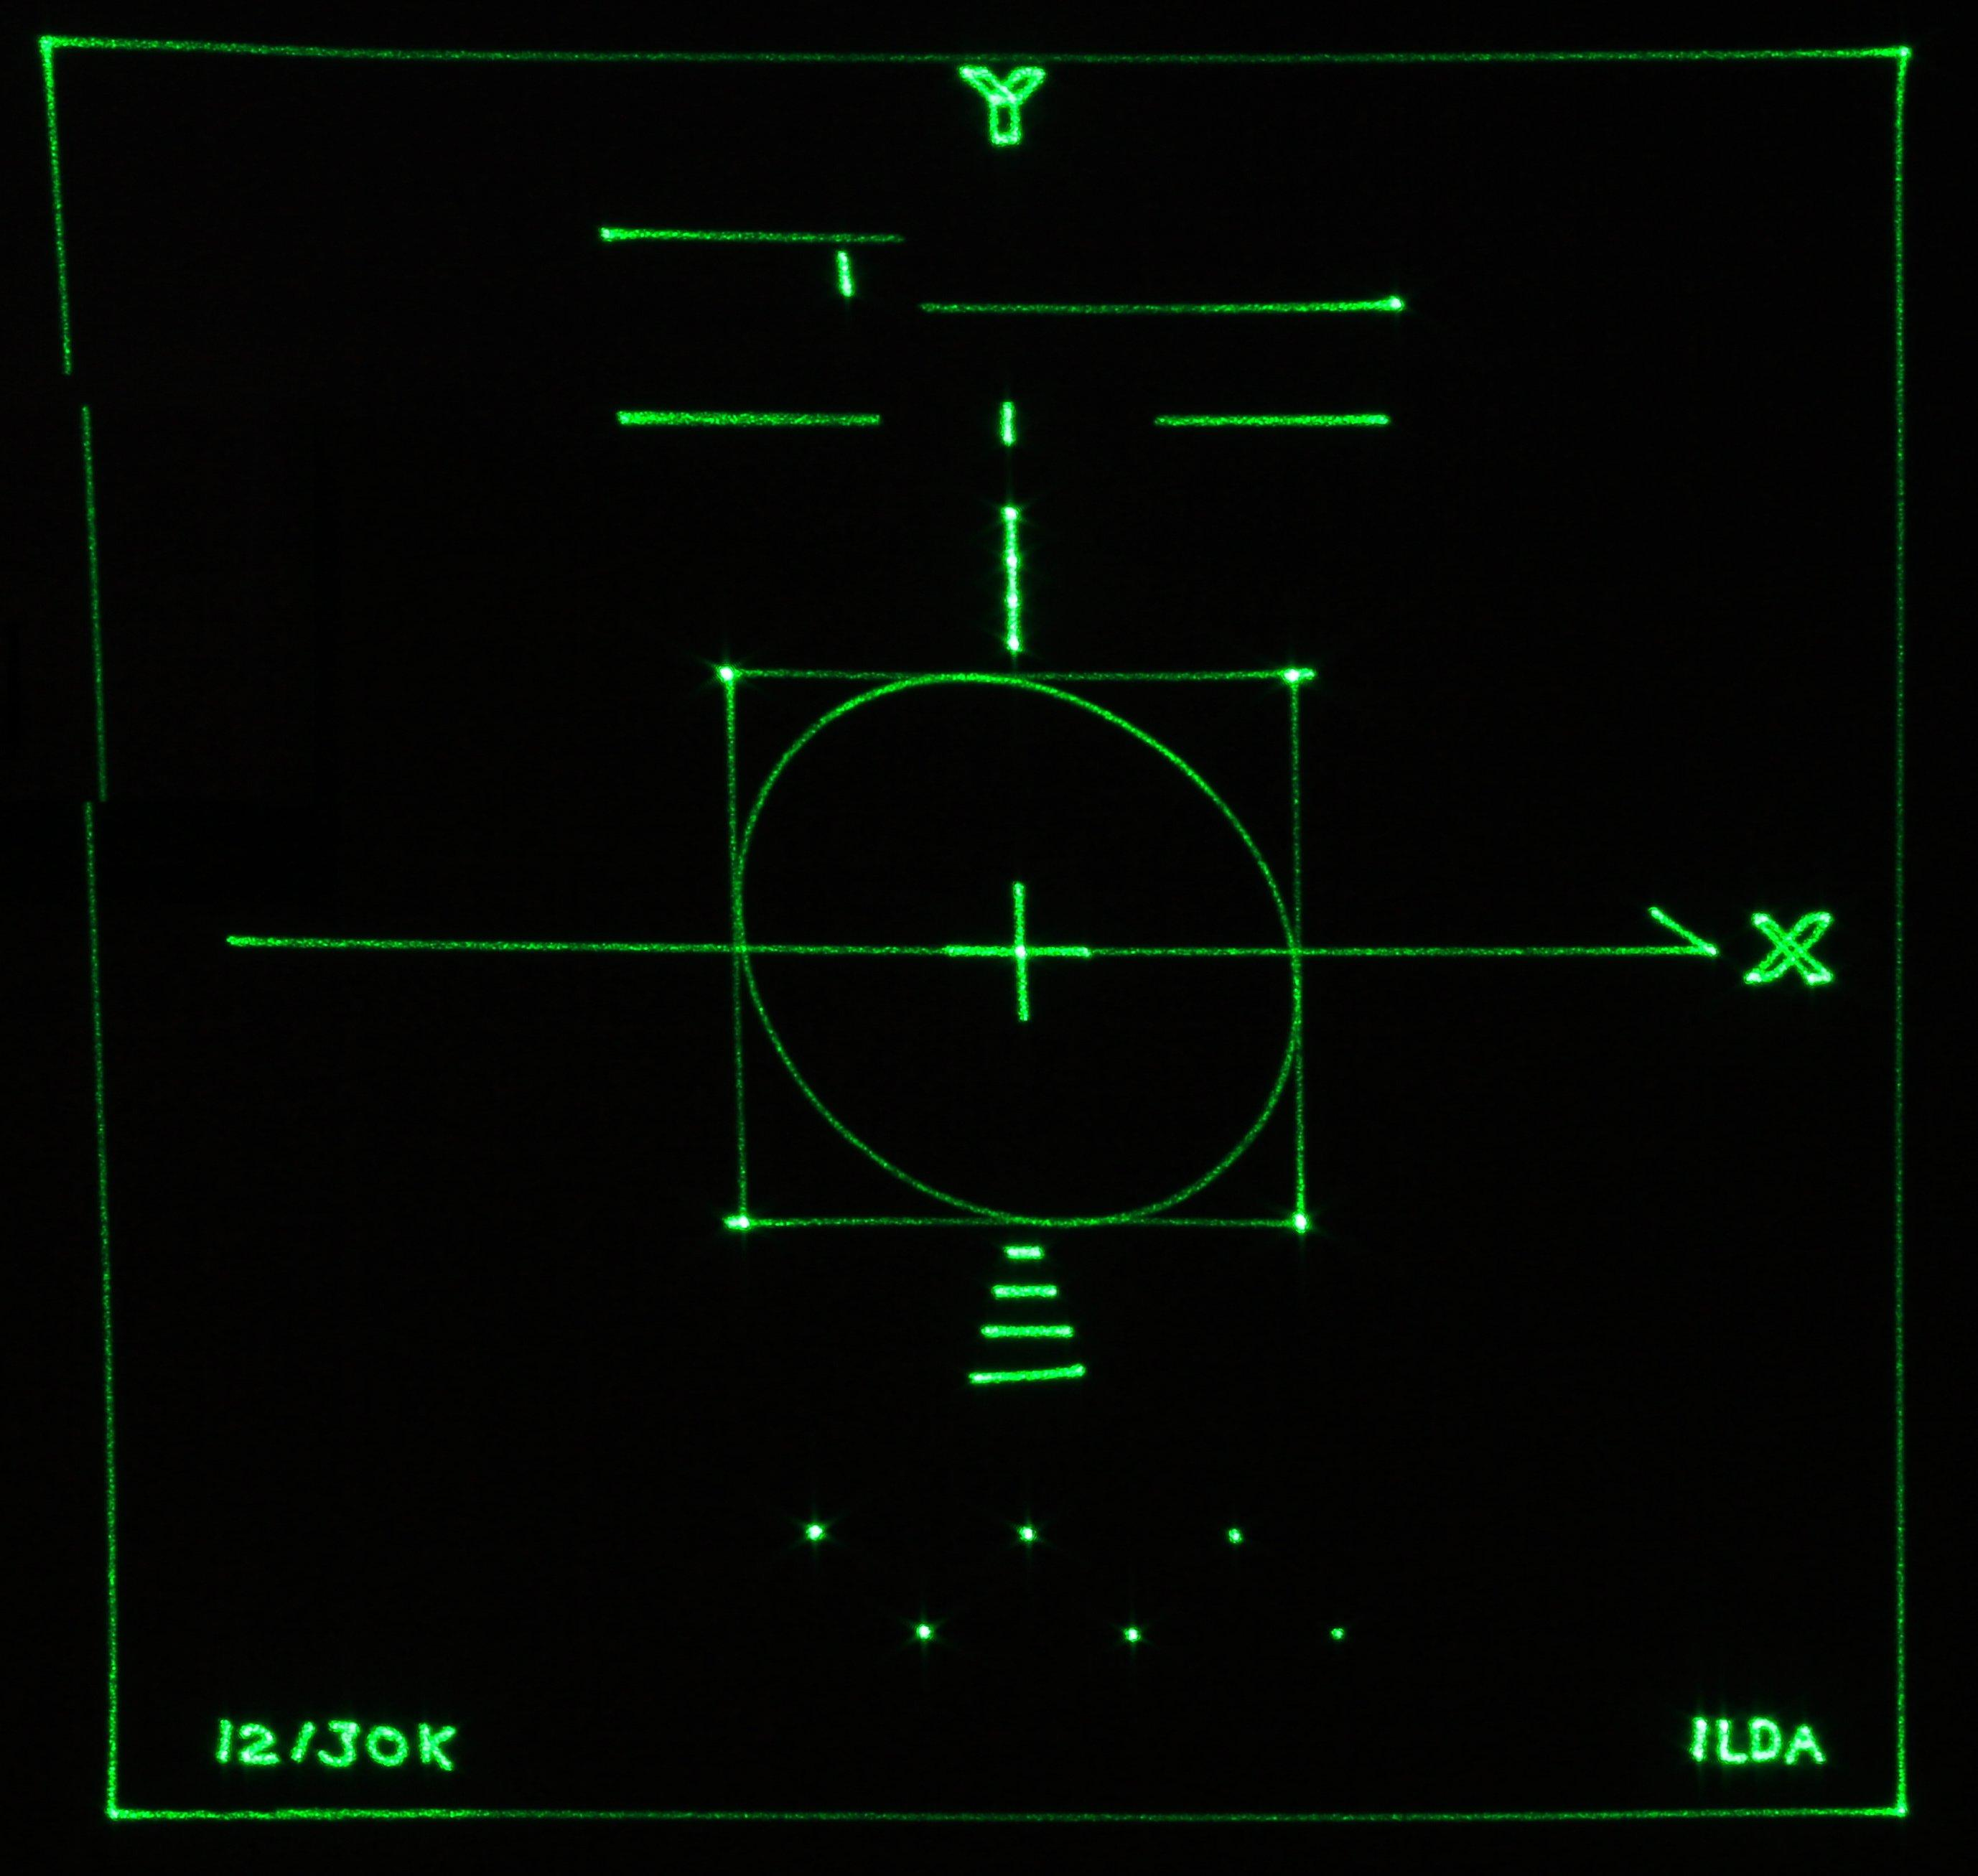
\includegraphics[width=\textwidth]{images/comp/custom_proj_10k.jpg}
                \caption{Laser Drawer}
                \label{fig:proj_test_custom}
        \end{subfigure}
        \begin{subfigure}[b]{0.5\textwidth}
                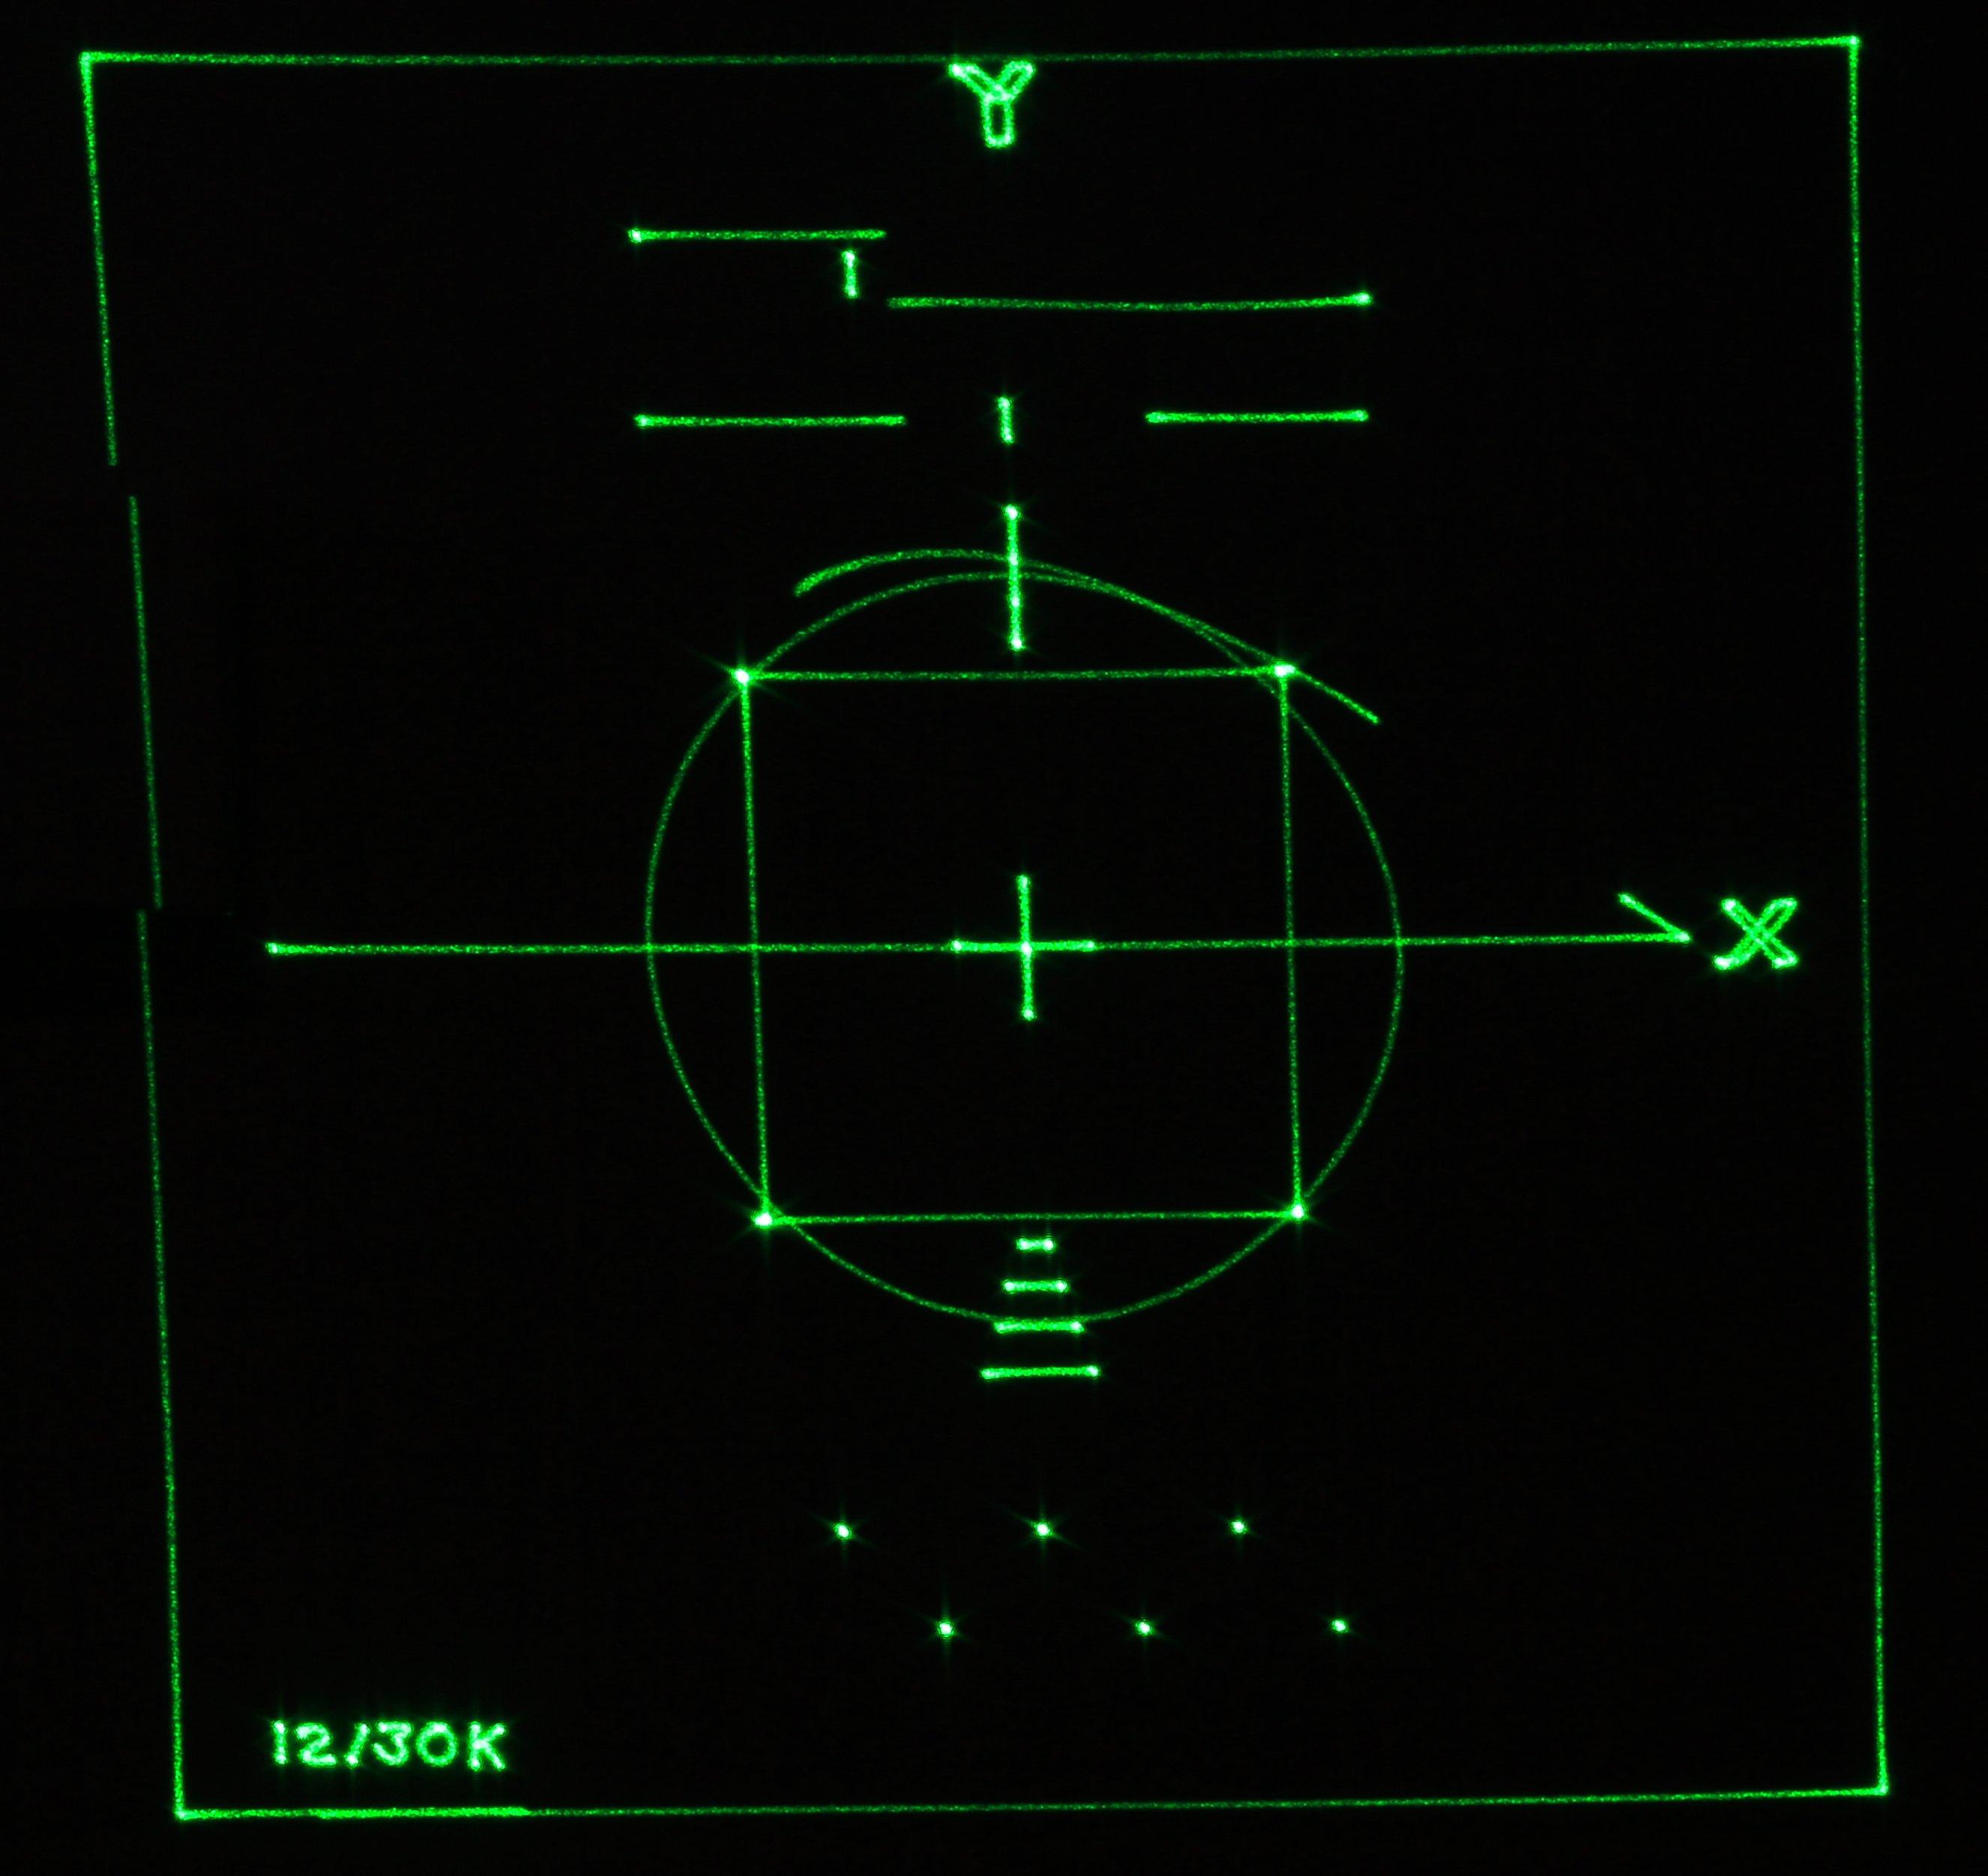
\includegraphics[width=\textwidth]{images/comp/galaxy_proj_10k.jpg}
                \caption{Galaxy}
                \label{fig:proj_test_galaxy}
        \end{subfigure}       
	\end{bigcenter}
\begin{fr}
\caption{Projection au laser à 12\unit{kpps}}
\end{fr}
\begin{en}
\caption{Laser projection at 12\unit{kpps}}
\end{en}
\label{fig:proj_test}
\end{figure}

\clearpage

\begin{appendices}
\begin{fr}
\section{Schéma électronique}
\end{fr}

\begin{en}
\section{Electronic Schematics}
\end{en}


\begin{fr}
\paragraph*{} La figure \ref{schema_beta} présente le montage du prototype réalisé. Ce schéma fonctionne, néanmoins il souffre de quelques défauts.
Tout d'abord, il n'y a pas de protection contre les court-circuits en sortie.
Les AOP risquent donc d'être endommagés lors d'un mauvais branchement ou d'un défaut de l'équipement relié.

Le convertisseur DC/DC 5\unit{V} isolé permet d'inverser la tension d'alimentation.
Grâce à ce composant et aux AOP rail-to-rail, le montage peut être alimenté par l'USB.
Toutefois, l'alimentation prélevé sur la carte son n'est que de $4,85\unit{V}$ et le convertisseur la transforme en $-4,95\unit{V}$, l'alimentation est alors dissymétrique.

Mais ces composants sont assez onéreux. On pourrait réduire les coûts, sans réduire la qualité, en prenant une alimentation ailleurs, sur l'alimentation des scanners à  l'intérieur du laser par exemple qui fournit généralement $+15\unit{V}$ et $-15\unit{V}$.
Dans ce cas, un double régulateur $+9\unit{V}/-9\unit{V}$ (LM7809 et LM7909) et des AOP types NE5532 (ou équivalents) sont suffisants.

Une autre limitation de ce montage est sa sensibilité à la capacité des longs câbles.
Lorsqu'un câble long ($> 50\unit{m}$) est utilisé, il ajoute une charge capacitive non négligeable et des oscillations parasites peuvent apparaître.
Il convient dans ce cas de rajouter des condensateurs de 220\unit{pF} dans la contre-réaction des AOP, en parallèle des résistances de 10\unit{k\Omega}.
\end{fr}

\begin{en}
The prototype schematic on figure  \ref{schema_beta} works but has some defects.
First it's not really ILDA compliant since the output isn't balanced.
Also there is no short circuit protection on outputs.
The op-amps could be damaged by a connection error or a hardware failure.

The board was powered by USB but there is only 4.85\unit{V} on the end and it's not enough for DC/DC converter to work properly.

It will be easier to use a DC/DC 5\unit{V} to 9\unit{V} converter.
In this case, we could choose better op-amp (not rail-to-rail, so cheaper) like NE5532.
\end{en}

\begin{fr}
\paragraph*{}
La figure \ref{fig:schema_rgb} présente un schéma amélioré permettant de piloter un laser RGB.
Les sorties sont symétrisées par des AOP et protégées des courts circuits par des résistances.
Des condensateurs dans la contre-réaction des AOP évitent les oscillations spontanées.


Le convertisseur DC/DC \texttt{XP-POWER IH0509S} possède une large plage de tension d'entrée (de $4,5\unit{V}$ à $9\unit{V}$) et une double tension de sortie régulée $+9\unit{V}/-9\unit{V}$ ce qui permet d'utiliser des AOP non rail-to-rail et donc moins onéreux et d'obtenir la tension régulée avec l'alimentation USB de $4,85\unit{V}$
J'ai choisi des NE5532 pour leurs performances audio et leur très bon rapport qualité/prix.
Les jumpers JP1 à JP6 sont des fils montés en surface pour faire des liaisons et éviter d'avoir un typon double face.
Les liaisons des jumpers sont représentées en jaune sur le schéma de la figure \ref{fig:schema_piste_composant} page \pageref{fig:schema_piste_composant}.

La figure \ref{fig:schema_piste_composant} page \pageref{fig:schema_piste_composant} présente le circuit électronique avec les composants pour référence.
La figure \ref{fig:typon} page \pageref{fig:typon} présente le typon.
Le tableau \ref{tab:comp_list} page \pageref{tab:comp_list} liste les composants utilisés.
\end{fr}

\begin{en}
There is an improved schematic on figure \ref{fig:schema_rgb} to drive a RGB laser.
On this, outputs are balanced and there are capacitors in the feedback loop of op-amp, so that spontaneous oscillations are avoided.
Some resistors on the output protect op-amp against short circuit.

The DC/DC converter \texttt{XP-POWER IH0509S} has a wide range of input voltage (from $4,5\unit{V}$ to $9\unit{V}$) and a dual regulated output.
Thus I can choose non-rail-to-rail and then cheaper op-amp.
I choose NE5532 for its good quality/price ratio and its good audio performances.
Jumpers JP1 to JP6 are on-board wires to avoid double face PCB.
The jumpers connections are drawn in yellow on the component implemantation schematic \ref{fig:schema_piste_composant} page \pageref{fig:schema_piste_composant}.

The figure \ref{fig:typon} shows the PCB and the table \ref{tab:comp_list} is the list of components.
\end{en}


\begin{figure}[ht]
\begin{bigcenter}
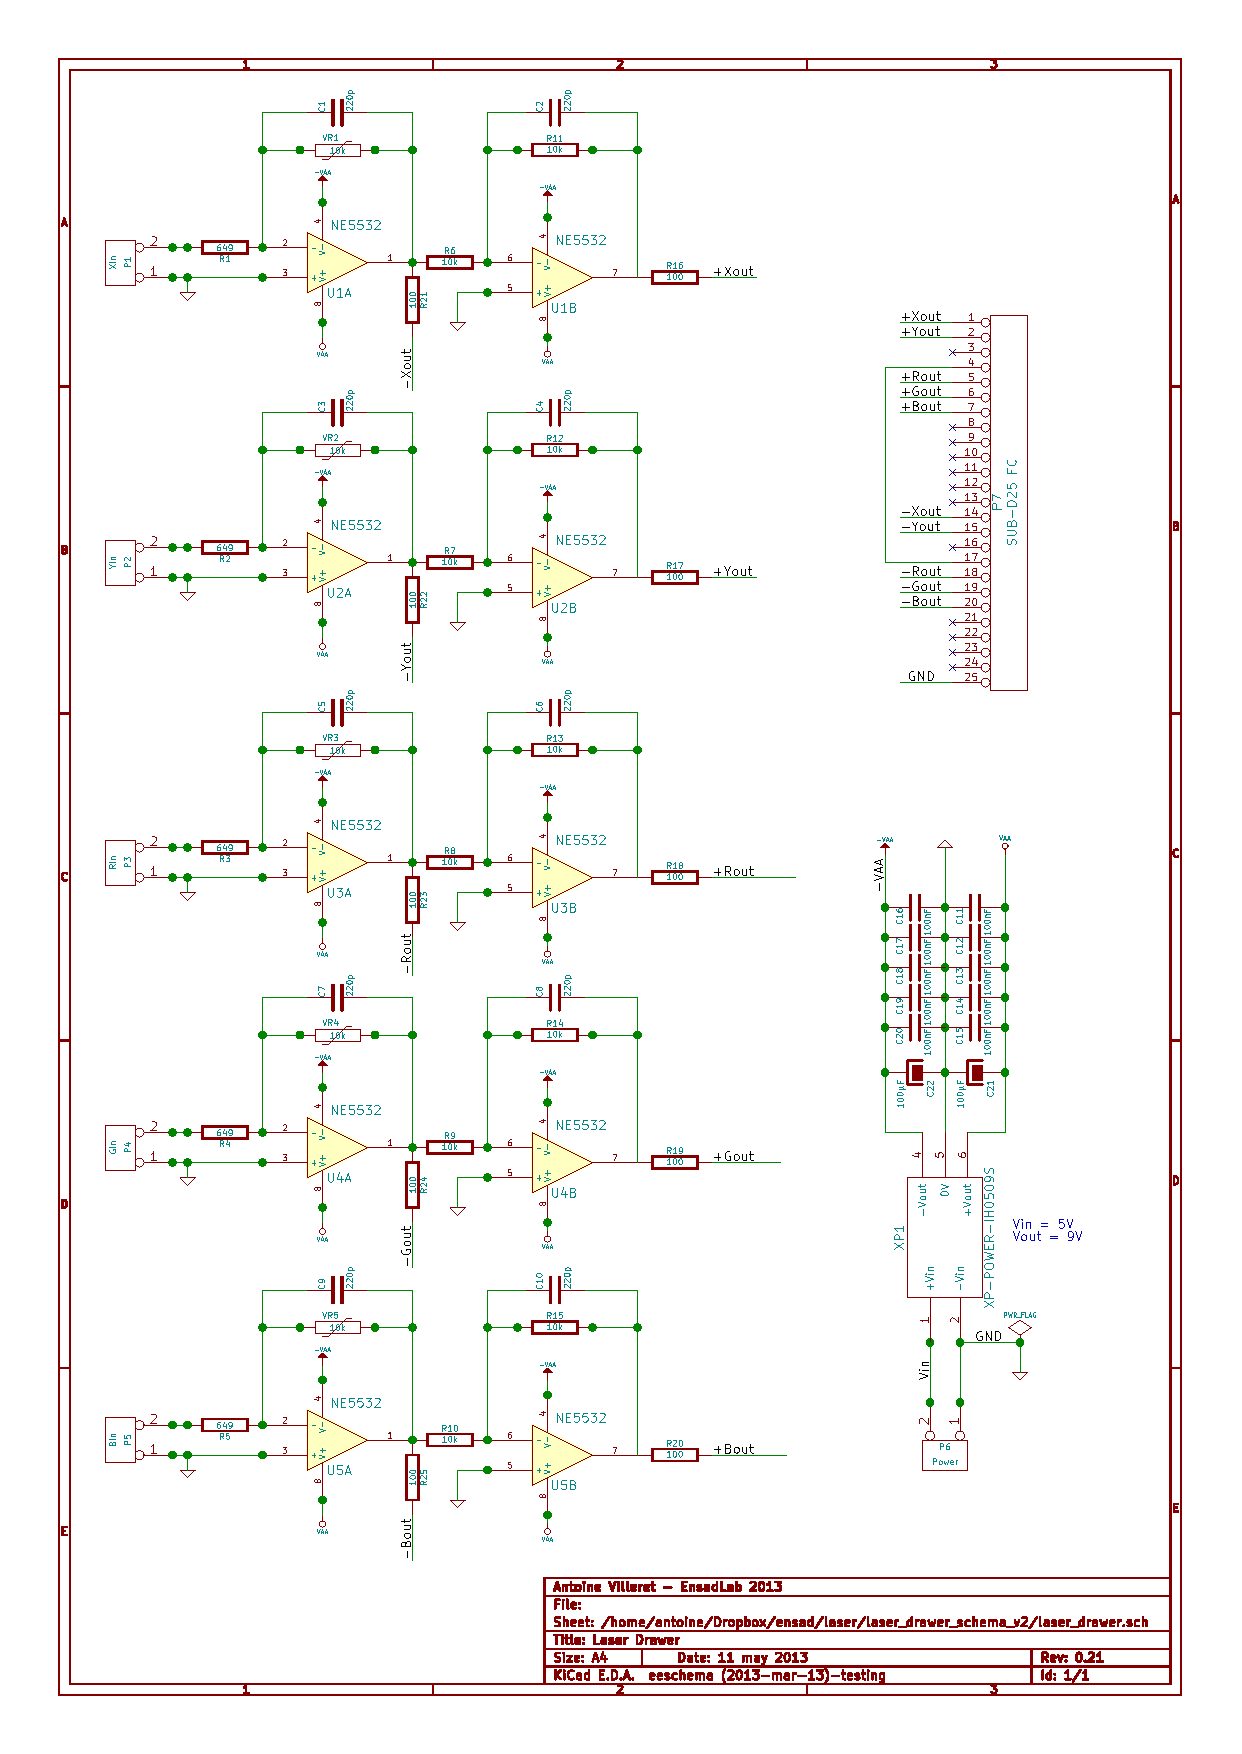
\includegraphics{../laser_drawer_schema/laser_drawer.pdf}
\end{bigcenter}
\begin{fr}
\caption{Schéma du prototype réalisé}
\label{schema_beta}
\end{fr}
\begin{en}
\caption{Prototype Schematic}
\label{schema_beta}
\end{en}
\end{figure}

\begin{figure}[ht]
\begin{bigcenter}
\vskip -120pt
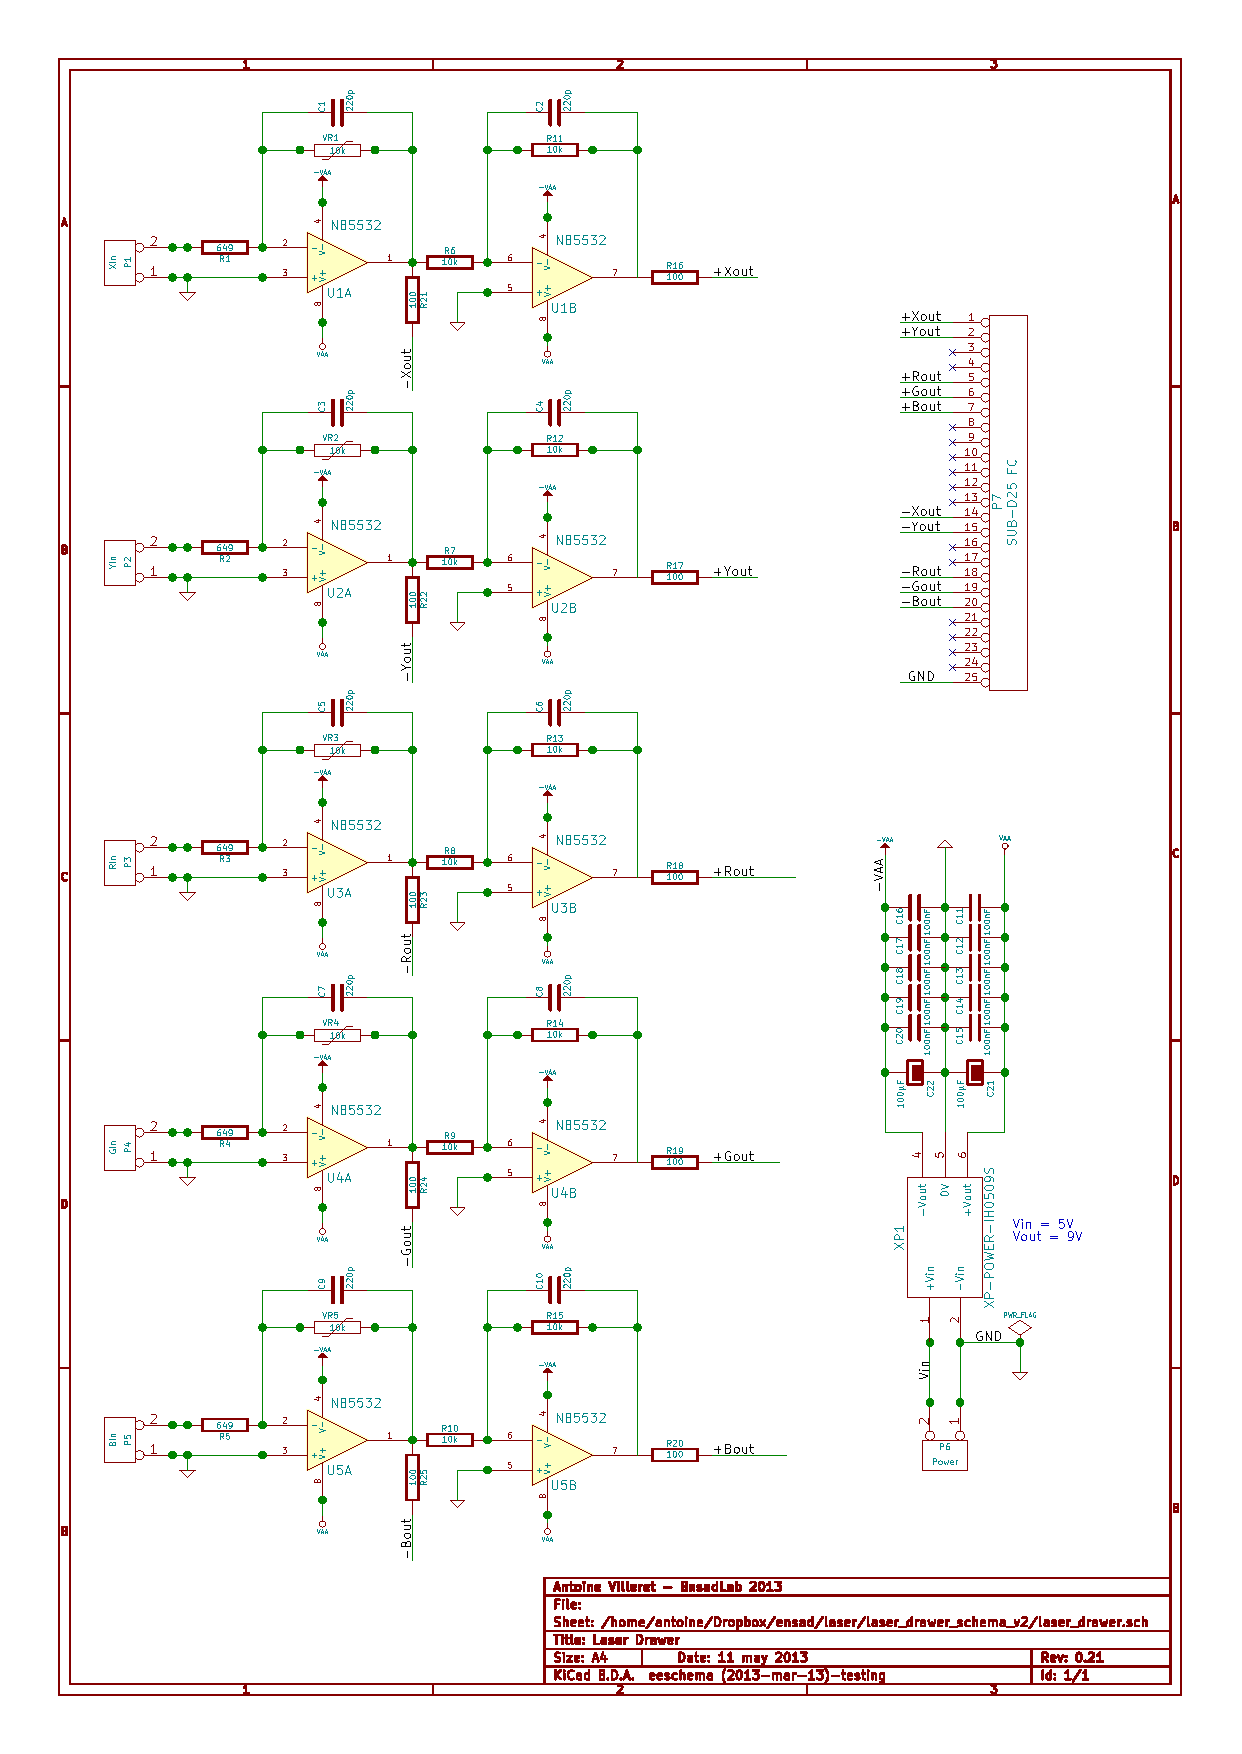
\includegraphics[scale=0.90]{../laser_drawer_schema_v2/laser_drawer.pdf}
\end{bigcenter}
\begin{fr}
\caption{Schéma de la version RGB symétrisée}
\label{fig:schema_rgb}
\end{fr}
\begin{en}
\caption{Balanced Output and 3 Color Channel Schematic}
\label{fig:schema_rgb}
\end{en}
\end{figure}

\begin{figure}[ht]
\begin{bigcenter}
\vskip -80pt
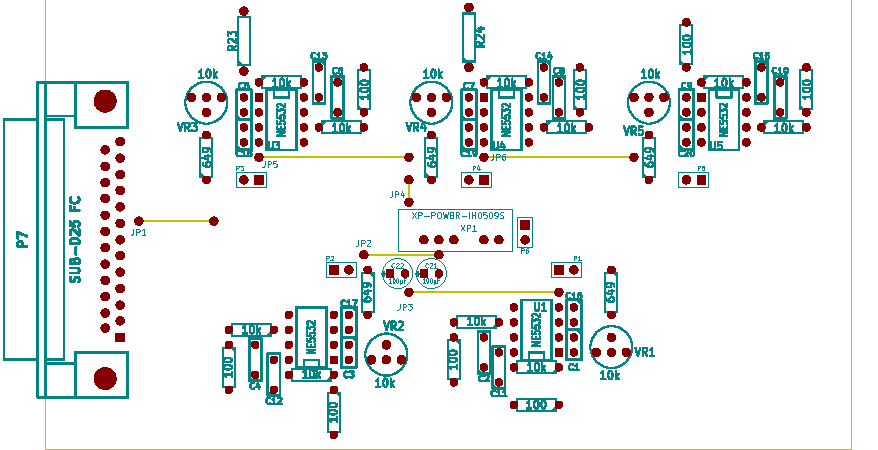
\includegraphics[scale=1,angle=0]{../laser_drawer_schema_v2/pdf/laser_drawer--brd.pdf}
\end{bigcenter}
\begin{fr}
\caption{Implantation des composants}
\label{fig:schema_piste_composant}
\end{fr}
\begin{en}
\caption{PCB}
\label{fig:schema_piste_composant}
\end{en}
\end{figure}

\begin{figure}[ht]
\begin{bigcenter}
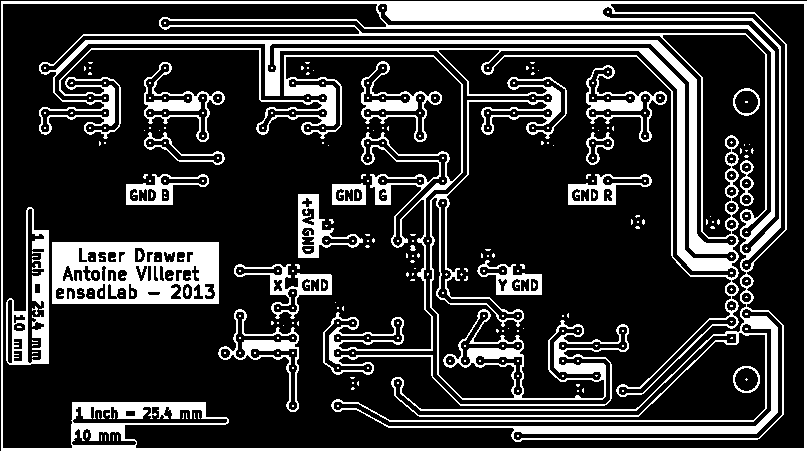
\includegraphics[scale=1]{../laser_drawer_schema_v2/pdf/laser_drawer-B_Cu.pdf}
\end{bigcenter}
\begin{fr}
\caption{Typon}
\label{fig:typon}
\end{fr}
\begin{en}
\caption{Offset Film}
\label{fig:typon}
\end{en}
\end{figure}

\begin{fr}
\begin{table}[h]
\centering
        \begin{tabular}{|l|l|l|l|}
            \hline 
            Ref. & Valeur & Quantité & ref. Farnell\\
            \hline
            C1 à C10 & $220\unit{pF}$ & 10 & \\
            \hline 
            C11 à C20 & $100\unit{nF}$ & 10 & \\
            \hline 
            C21, C22 & $100\unit{\mu F}$ & 2 & \\
            \hline  
            JP1 à JP6 & JUMPER & 6 & \\
            \hline 
            P1 à P6 & 2x1 PIN HEADER & 6 & \href{http://fr.farnell.com/jsp/search/productdetail.jsp?sku=9731148}{9731148}\\
            \hline 
            P7 & SUB-D25 FC & 1 & \href{http://fr.farnell.com/jsp/search/productdetail.jsp?sku=1099296}{1099296}\\
	        \hline    
            R1 à R5 & $649\unit{\Omega}$ & 5 & \\
            \hline
            R6 à R15 & $10\unit{k\Omega}$ & 10 & \\
            \hline 
            R16 à R25 & $100\unit{\Omega}$ & 10 & \\ 
            \hline 
            U1 à U5 & NE5532 & 5 & \href{http://fr.farnell.com/jsp/search/productdetail.jsp?sku=1106091}{1106091}\\
            \hline 
            VR1 à VR5 & $10\unit{k\Omega}$ trimer & 5 & \href{http://fr.farnell.com/jsp/search/productdetail.jsp?sku=9354301}{9354301}\\
            \hline 
            XP1 & XP-POWER IH0509S & 1 & \href{http://fr.farnell.com/jsp/search/productdetail.jsp?sku=8727880}{8727880}\\
            \hline
        \end{tabular}
    \caption{\label{tab:comp_list} Liste des composants utilisés dans le circuit}
\end{table}
\end{fr}

\begin{en}
\begin{table}[h]
\centering
        \begin{tabular}{|l|l|l|l|}
            \hline 
            Ref. & Value & Quantity & Ref. Farnell \\
            \hline
            C1 à C10 & $220\unit{pF}$ & 10 & \\
            \hline 
            C11 à C20 & $100\unit{nF}$ & 10 & \\
            \hline 
            C21, C22 & $100\unit{\mu F}$ & 2 & \\
            \hline  
            JP1 à JP6 & JUMPER & 6 & \\
            \hline 
            P1 à P6 & 2x1 PIN HEADER & 6 & \href{http://fr.farnell.com/jsp/search/productdetail.jsp?sku=9731148}{9731148}\\
            \hline 
            P7 & SUB-D25 FC & 1 & \href{http://fr.farnell.com/jsp/search/productdetail.jsp?sku=1099296}{1099296}\\
	        \hline    
            R1 à R5 & $649\unit{\Omega}$ & 5 & \\
            \hline
            R6 à R15 & $10\unit{k\Omega}$ & 10 & \\
            \hline 
            R16 à R25 & $100\unit{\Omega}$ & 10 & \\ 
            \hline 
            U1 à U5 & NE5532 & 5 & \href{http://fr.farnell.com/jsp/search/productdetail.jsp?sku=1106091}{1106091}\\
            \hline 
            VR1 à VR5 & $10\unit{k\Omega}$ trimer & 5 & \href{http://fr.farnell.com/jsp/search/productdetail.jsp?sku=9354301}{9354301}\\
            \hline 
            XP1 & XP-POWER IH0509S & 1 & \href{http://fr.farnell.com/jsp/search/productdetail.jsp?sku=8727880}{8727880}\\
            \hline
        \end{tabular}
    \caption{\label{tab:comp_list} Bill of materials}
    \end{table}
\end{en}
	
\clearpage
        
\begin{fr}
\section{Législation sur les lasers}
\label{sec:legislation}
Les lasers peuvent être dangereux.
Une forte quantité de lumière cohérente concentrée sur une petite surface fait monter ponctuellement la température.
C'est pour cela que les lasers sont utilisés pour découper des matériaux.
Mais cette propriété représente un danger potentiel, à la fois pour les personnes mais aussi pour les biens.
On peut être brûlé par un laser et les yeux sont également très sensibles.
Par exemple, il est possible d'allumer une cigarette avec un faisceau laser de 5\unit{W}.
Il est donc nécessaire de prendre des précautions dans la mise en \oe uvre d'un laser.
Tout cela est encadré par des lois et décrets qui parfois sont difficiles à appliquer.

Cette annexe tente d'éclaircir les mesures réglementaires et de les relativiser par rapport à l'utilisation que l'on fait des lasers.
\end{fr}

\begin{en}
\section{Legal and security issues with the lasers}
\label{sec:legislation}
Lasers could be dangerous.
A high level of coherent light concentrated on a small surface heats quickly.
That is why we use lasers to cut materials.
But this property is also dangerous, both for things and people.
A 5\unit{W} laser can burn the skin or lighten a cigarette.

The laws define some restrictions that could be difficult to follow.
I will try to clarify those and to relativise according to what we are doing with lasers.
\end{en}


\begin{fr}
\subsection*{Les risques}
	Les lasers peuvent brûler la peau et surtout la rétine. Les lésions rétiniennes sont irréversibles.
	On peut donc devenir définitivement aveugle en regardant un laser à l'\oe il nu.
	
	Les lasers de classe 4 peuvent déclencher un incendie. Si le faisceau reste fixe sur une surface inflammable, elle s'enflamme rapidement.
	
	Pour que l'exposition reste sans danger, la quantité d'énergie reçue ne doit pas dépasser le seuil de l'Exposition Maximale Permise (EMP).
	L'EMP est définie comme le dixième de la dose qui a une chance sur deux de produire une lésion dans les conditions les plus défavorables.
Elle est mesurée sur la cornée ou sur la peau pour une longueur d'onde et un temps d'exposition donnés.
L'EMP est expimée en \unit{W/cm^2} ou \unit{J/cm^2}.
Sur la figure \ref{fig:mpe-watt}, on voit que l'exposition continue de la cornée à un laser visible est dangeurse à partir d'1\unit{mW}.

Les lasers sont également dangereux pour l'aviation.
Si les avions sont toujours suffisamment loin pour que le laser ne les endommage pas il est en revanche possible que les pilotes soient éblouis.
\end{fr}

\begin{en}
\subsection*{The risks}
Lasers can burn the skin and the retina.
Retina's injuries are irrevocable.
Man can become blind by directly looking into a laser diode.
Class 4 lasers can easily trig a fire.

To be safe, the exposure shouldn't go above the Maximum Permissible Exposure (MPE).
MPE is defined as the tenth of the dose which has half chance to make an irrevocable injury.
This is measured on the cornea or on the skin for a given wave length and exposure time.
MPE used to be expressed in \unit{W/cm^2} ou \unit{J/cm^2}.
Figure \ref{fig:mpe-watt} shows the continuous exposition of cornea to visible laser is dangerous above 1\unit{mW}.

Lasers could also be dangereous for aviation.
Even if the planes fly high enough to not be damaged by a laser beam, pilot could be dazzled.
\end{en}

\begin{fr}
\begin{figure}
        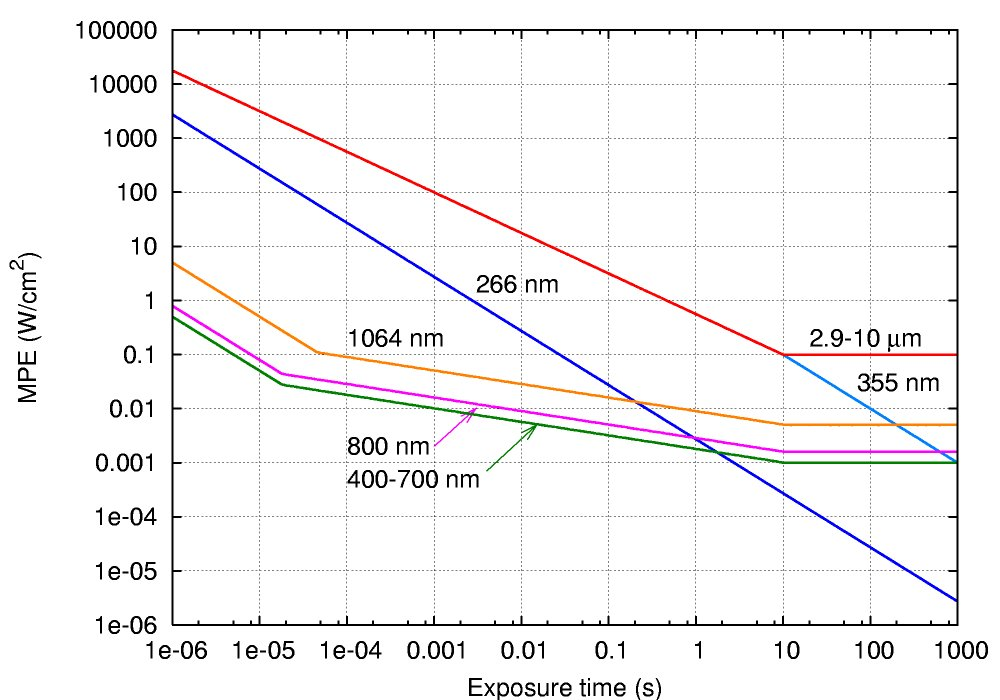
\includegraphics[width=\textwidth]{images/IEC60825_MPE_W_s.jpg}
                \caption{MPE pour différentes longueurs d'onde (source : Wikipedia)}
        \label{fig:mpe-watt}
\end{figure}
\end{fr}
        
\begin{en}
        \begin{figure}
        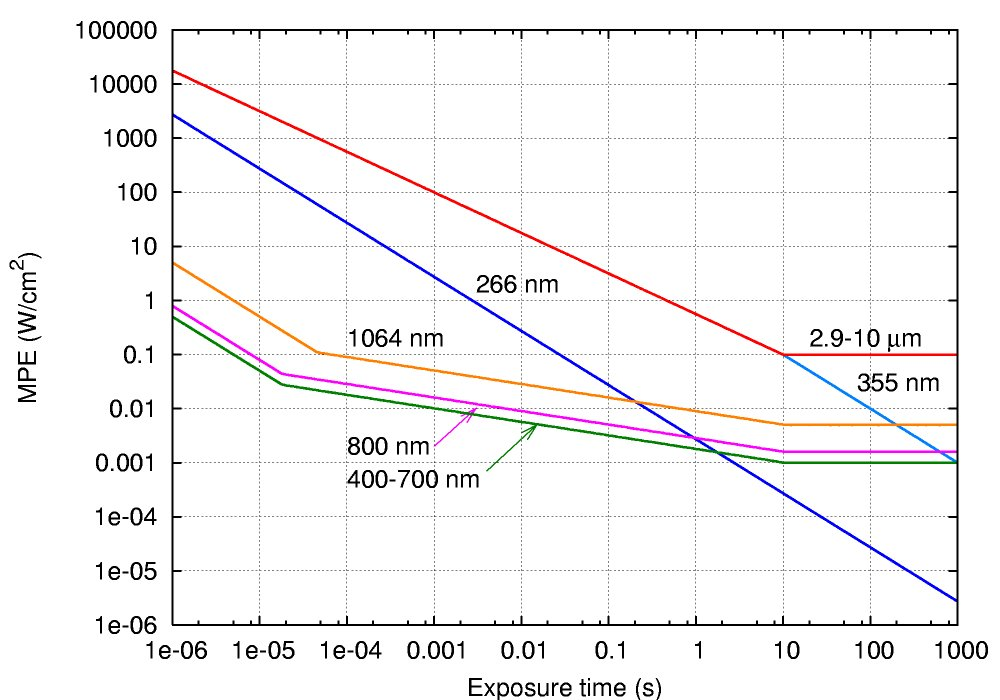
\includegraphics[width=\textwidth]{images/IEC60825_MPE_W_s.jpg}
                \caption{MPE for several wavelenght (source : Wikipedia)}
        \label{fig:mpe-watt}
        \end{figure}
\end{en}


\newgeometry{hmargin=3cm}
\begin{fr}
\begin{table}
\begin{bigcenter}
	\begin{tabular}{|l|p{0.9\textwidth}|}
\hline 
Classe 1 & lasers sans danger, à condition de les utiliser dans leurs conditions raisonnables prévisibles (exemples : imprimantes, lecteurs de CD-ROM et lecteurs de DVD). \\
\hline
Classe 1M & lasers dont la vision directe dans le faisceau, notamment à l’aide d’instrument optiques, peut être dangereuse. \\
\hline
Classe 2 & lasers qui émettent un rayonnement visible dans la gamme de longueur de 400 à 700 nm. La protection de l’œil est normalement assurée par les réflexes de défense comprenant le réflexe palpébral, clignement de la paupière (par exemple, des lecteurs de code-barres). \\
\hline
Classe 2M & lasers qui émettent un rayonnement visible dans la gamme de longueur de 400 à 700 nm. Lasers dont la vision directe dans le faisceau, notamment à l’aide d’instrument optiques, peut être dangereuse (exemples : loupes et télescopes). \\
\hline
Classe 3A & lasers dont l’exposition directe dépasse l’EMP (Exposition Maximale Permise) pour l’œil, mais dont le niveau d’émission est limité à cinq fois la LEA (Limite d’Émission Accessible) des classes 1 et 2. \\
\hline
Classe 3B & laser dont la vision directe du faisceau est toujours dangereuse. La vision de réflexions diffuses est normalement sans danger. \\
\hline
Classe 4 & lasers qui sont aussi capables de produire des réflexions diffuses dangereuses. Ils peuvent causer des dommages sur la peau et peuvent également constituer un danger d’incendie. Leur utilisation requiert des précautions extrêmes. \\
\hline

	\end{tabular}
	\end{bigcenter}
	\caption{\label{tab:laser_classification} Classification des lasers (source : Wikipedia)}
\end{table}	
\end{fr}

\begin{en}
\begin{table}
\begin{bigcenter}
	\begin{tabular}{|l|p{0.9\textwidth}|}
\hline 
Class 1 & A Class 1 laser is safe under all conditions of normal use. This means the maximum permissible exposure (MPE) cannot be exceeded when viewing a laser with the naked eye or with the aid of typical magnifying optics (e.g. telescope or microscope). To verify compliance, the standard specifies the aperture and distance corresponding to the naked eye, a typical telescope viewing a collimated beam, and a typical microscope viewing a divergent beam. It is important to realize that certain lasers classified as Class 1 may still pose a hazard when viewed with a telescope or microscope of sufficiently large aperture. For example, a high-power laser with a very large collimated beam or very highly divergent beam may be classified as Class 1 if the power that passes through the apertures defined in the standard is less than the AEL for Class 1; however, an unsafe power level may be collected by a magnifying optic with larger aperture. \\
\hline
Class 1M & A Class 1M laser is safe for all conditions of use except when passed through magnifying optics such as microscopes and telescopes. Class 1M lasers produce large-diameter beams, or beams that are divergent. The MPE for a Class 1M laser cannot normally be exceeded unless focusing or imaging optics are used to narrow the beam. If the beam is refocused, the hazard of Class 1M lasers may be increased and the product class may be changed. A laser can be classified as Class 1M if the power that can pass through the pupil of the naked eye is less than the AEL for Class 1, but the power that can be collected into the eye by typical magnifying optics (as defined in the standard) is higher than the AEL for Class 1 and lower than the AEL for Class 3B. \\
\hline
Class 2 & A Class 2 laser is safe because the blink reflex will limit the exposure to no more than 0.25 seconds. It only applies to visible-light lasers (400–700 nm). Class-2 lasers are limited to 1 mW continuous wave, or more if the emission time is less than 0.25 seconds or if the light is not spatially coherent. Intentional suppression of the blink reflex could lead to eye injury. Many laser pointers and measuring instruments are class 2. \\
\hline
Class 2M & A Class 2M laser is safe because of the blink reflex if not viewed through optical instruments. As with class 1M, this applies to laser beams with a large diameter or large divergence, for which the amount of light passing through the pupil cannot exceed the limits for class 2. \\
\hline
Class 3R & A Class 3R laser is considered safe if handled carefully, with restricted beam viewing. With a class 3R laser, the MPE can be exceeded, but with a low risk of injury. Visible continuous lasers in Class 3R are limited to 5 mW. For other wavelengths and for pulsed lasers, other limits apply \\
\hline
Class 3B & A Class 3B laser is hazardous if the eye is exposed directly, but diffuse reflections such as those from paper or other matte surfaces are not harmful. The AEL for continuous lasers in the wavelength range from 315 nm to far infrared is 0.5 W. For pulsed lasers between 400 and 700 nm, the limit is 30 mJ. Other limits apply to other wavelengths and to ultrashort pulsed lasers. Protective eyewear is typically required where direct viewing of a class 3B laser beam may occur. Class-3B lasers must be equipped with a key switch and a safety interlock. Class 3B lasers are used inside CD and DVD writers, although the writer unit itself is class 1 because the laser light cannot leave the unit. \\
\hline
Class 4 & Class 4 is the highest and most dangerous class of laser, including all lasers that exceed the Class 3B AEL. By definition, a class 4 laser can burn the skin, or cause devastating and permanent eye damage as a result of direct, diffuse or indirect beam viewing. These lasers may ignite combustible materials, and thus may represent a fire risk. These hazards may also apply to indirect or non-specular reflections of the beam, even from apparently matte surfaces—meaning that great care must be taken to control the beam path. In most states it is illegal to sell preassembled class 4 lasers, however a citizen can construct a class 4 laser for personal use. Class 4 lasers must be equipped with a key switch and a safety interlock. Most industrial, scientific, military, and medical lasers are in this category. \\
\hline

	\end{tabular}
	\end{bigcenter}
	\caption{\label{tab:laser_classification} Laser classification (source : Wikipedia)}
\end{table}	
\end{en}
\restoregeometry{}


\begin{fr}
\subsection*{Réglementation}

Les lasers sont classés selon leur dangerosité (cf. table \ref{tab:laser_classification}).
Une première classification en chiffre romain ne prenait en compte que la puissance de la source.
Cette classification a été révisée en 2007 pour adopter une numérotation en chiffre arabe qui traduit toujours la dangerosité du laser mais elle prend en compte plus de paramètres comme la longueur d'onde ou la divergence (la taille de la tâche en fonction de la distance).

Les lasers de classe 3 et 4, utilisables exclusivement en plein air, sont mis en \oe uvre par un technicien compétent et formé aux risques spécifiques des lasers. 
\footnote{D'après le Journal Officiel de la République Française numéro 0039 du 16 février 2010, text 9}

Face à cette dangerosité, la législation impose des dispositifs de coupure automatique du faisceau en cas de défaillance du système.
Sur certains lasers on trouve un système qui coupe la diode si l'aire de balayage n'est pas suffisamment grande. 
Plus l'air de balayage est grande, moins le faisceau reste longtemps au même endroit et donc moins il est dangereux. 
Mais ce genre de dispositif est extrêmement contraignant puisqu'il n'est plus possible de dessiner des formes arbitraires 
même si des précautions sont prises ailleurs (surface de projection ignifugée, cône de projection inaccessible aux personnes\dots).
\end{fr}

\begin{en}
\subsection*{The law}
Lasers are classified according to their dangerousity (see table \ref{tab:laser_classification}).
The first classification in roman numbers takes only the diode power into account.
The 2007 revision takes also the wavelength and the divergence into account.

Laser from class 3 and above could only be used outdoor.
Only a qualified technician could manipulate the laser, but I can't find any compagny in France that delivers an agreement for animation lasers.
People have to learn laser safety themselves and take their responsability.

Due to this dangereousity, laser must have a security system to cut the beam if a failure occurs.
On some new lasers, the diode is switched off if the scanning area is not wide enough.
The bigger the scanning area is, the less the beam stay on the same place, so the less it is dangerous.
But with such a system we can't draw arbitrary patterns with laser even if we take compensatory arrangement like constraining beam or a fireproofed projection screen.

\end{en}

\begin{fr}
\subsection*{La pratique}
Dans la pratique cette législation est très contraignante et surtout peut faire peur aux personnes responsables.
Il est donc nécessaire d'expliquer les risques et les mesures de sécurité mises en \oe uvre.
Dès lors que l'on utilise un laser de classe 3 ou 4, il faut éviter autant que possible de balayer les spectateurs.
Si, malgré les risques, on souhaite tout de même balayer une zone où le public est présent, 
il faut s'assurer que la puissance reçu par le public est inférieure à l'EMP.
\end{fr}

\begin{en}
\subsection*{In practice}
In practice, the laws are very restrictive and moreover they can afraid technical director if they are not explained properly.
As soon as we use a Class 3 or above laser, audience scanning should be avoided.
If it is really needed to scan an area accessible to people, we must take some special measures to be sure that the audience exposure is below the MPE.
%~ mesures compensatoires., prendre des mesures
\end{en}

\begin{fr}
Robert Henke pour \textit{Fragiles Territoires} utilise des lasers de classe 4 en intérieur. 
Pour cela, il a mis en place une barrière physique qui, si elle est franchie, coupe automatiquement les lasers. 
Les personnes ne peuvent donc jamais entrer dans la zone de balayage.
De longues discussions ont été nécessaires avant que le dispositif de sécurité ne soit approuvé.  
\end{fr}

\begin{en}
Robert Henke uses class 4 laser indoor for \textit{Fragiles Territoires}. 
He had to setup an IR barrier to cut of all lasers if someone enters in the forbidden area.
Thus nobody can be reached by the laser beam.
He had to go through a lot of discussions before this was approved.
\end{en}

\begin{fr}
Pour \textit{Enseigne} de Samuel Bianchini, le laser de 8\unit{W} est contraint par une fenêtre noire en aluminium.
À travers cette fenêtre, le faisceau ne peut qu'atteindre sa cible : la façade d'un immeuble situé à 250\unit{m}.
Si le faisceau sort de la fenêtre, il est dissipé par le métal noir qui ne peut fondre même si le faisceau reste fixe longtemps.
\end{fr}

\begin{en}
For \textit{Sign} by Samuel Bianchini, the laser is constrained into a small black metal window.
Through this window the laser beam can only reach its target : a front of a building 250\unit{m} far.
If in any case the beam leave the window, the surrounding metal absorbs it.
\end{en}

\begin{fr}
Quant à Robin Fox, dans son show il balaye le public qui peut recevoir le laser dans les yeux.
Il ne semble pas inconscient des dangers mais ignore que son laser (classe 3, 532\unit{nm} 350\unit{mW}) est interdit d'utilisation en intérieur, du moins en France.
\end{fr}

\begin{en}
Concerning Robin Fox, he places the laser projector in front of the audience so that the beam can reach our eyes easily.
He seems to be aware of the laser's hazards but doesn't know his laser is forbidden indoor, in France at least.
\end{en}

\begin{fr}
\section{Crédit image}
        
L'image \ref{fig:fluidic} est reproduite avec l'aimable autorisation de White Void.

L'image \ref{fig:laser_forest} est reproduite avec l'aimable autorisation de Marshmallow Laser Feast.

L'image \ref{fig:henke}  est reproduite avec l'aimable autorisation de Robert Henke.

J'ai personnellement réalisé les photos \ref{fig:bianchini} et   \ref{fig:fox}.

Les demandes d'autorisation de reproduction pour les autres photos sont restées sans suite. 
J'ai décidé de tout de même les reproduire pour illustrer mon dossier.
Elles peuvent être retirées sur simple demande des auteurs.
\end{fr}

\begin{en}
        \section{Image credit}
        
        Picture \ref{fig:laser_forest} is reproduced with courtesy of Marshmallow Laser Feast. \\
        Picture \ref{fig:fluidic} is reproduced with courtesy of White Void. \\
        Picture  \ref{fig:henke} is reproduced with courtesy of Robert Henke himself. \\        
        Pictures \ref{fig:bianchini} and \ref{fig:fox} are mine. \\
        
        Other pictures are reproduced without courtesy because I received no answer from their owners.
        Eventhough I decided to reproduce them to illustrate this report.
        I will remove them if author claims.
        
\end{en}

\end{appendices}

\end{document}
